\documentclass[10pt, twoside]{book}

%%% preambulo
\input ../preambulo.tex
\input ../preambulo_counters.tex
\input ../preambulo_python.tex

\makeindex

\begin{document}

\frontmatter

\title{Cálculo I}
\author{Pedro H A Konzen}
\date{\today}
\maketitle

% ficha catolográfica
\ifisbook
~
\vspace{4in}
\hrule
Konzen, Pedro Henrique de Almeida \\
\indent\hspace{2em}Calculo I: notas de aula / Pedro Henrique de Almeida Konzen. --{\the\year}. Porto Alegre.- {\the\year}. \\
\indent\hspace{2em}"Esta obra é uma edição independente feita pelo próprio autor." \\
\indent\hspace{2em}1. Algoritmos computacionais. 2. Programação de computadores. 3. Linguagem Python. \\
\hrule
\vspace{1cm}
\begin{center}
  \textit{Licença}\\CC-BY-SA 4.0.
\end{center}
\fi

% licença
\chapter*{Licença}\label{licenca}
\addcontentsline{toc}{chapter}{Licença}

Este texto é disponibilizado sob a Licença Atribuição-CompartilhaIgual 4.0 Internacional Creative Commons. Para visualizar uma cópia desta licença, visite 
\begin{center}
  \url{http://creativecommons.org/licenses/by-sa/4.0/deed.pt\_BR} 
\end{center}
ou mande uma carta para Creative Commons, PO Box 1866, Mountain View, CA 94042, USA.




\chapter*{Prefácio}\label{prefacio}
\addcontentsline{toc}{chapter}{Prefácio}

O site \href{https://www.notaspedrok.com.br}{notaspedrok.com.br} é uma plataforma que construí para o compartilhamento de minhas notas de aula. Essas anotações feitas como preparação de aulas é uma prática comum de professoras/es. Muitas vezes feitas a rabiscos em rascunhos com validade tão curta quanto o momento em que são concebidas, outras vezes, com capricho de um diário guardado a sete chaves. Notas de aula também são feitas por estudantes - são anotações, fotos, prints, entre outras formas de registros de partes dessas mesmas aulas. Essa dispersão de material didático sempre me intrigou e foi o que me motivou a iniciar o site.

Com início em 2018, o site contava com apenas três notas incipientes. De lá para cá, conforme fui expandido e revisando os materais, o site foi ganhando acessos de vários locais do mundo, em especial, de países de língua portugusa. No momento, conta com 13 notas de aula, além de minicursos e uma coleção de vídeos e áudios.

As notas de \emph{Algoritmos e Programação I} fazem uma introdução a algoritmos e programação de computadores com a linguagem {\python}. É pensada para estudantes de cursos de matemática e áreas afins.

Aproveito para agradecer a todas/os que de modo assíduo ou esporádico contribuem com correções, sugestões e críticas. ;-)

\begin{flushright}
  Pedro H A Konzen\\\url{https://www.notaspedrok.com.br}
\end{flushright}




% toc
\ifishtml
\clearpage
\phantomsection
\addcontentsline{toc}{chapter}{Conteúdo}
\fi
\tableofcontents

\mainmatter

%Este trabalho está licenciado sob a Licença Atribuição-CompartilhaIgual 4.0 Internacional Creative Commons. Para visualizar uma cópia desta licença, visite http://creativecommons.org/licenses/by-sa/4.0/deed.pt_BR ou mande uma carta para Creative Commons, PO Box 1866, Mountain View, CA 94042, USA.

\chapter{Limites}\label{cap_lim}
\thispagestyle{fancy}

\section{Noção de limites}

Seja $f$ uma função definida em um intervalo aberto em torno de um dado ponto $x_0$, exceto talvez em $x_0$. Quando o valor de $f(x)$ é arbitrariamente próximo de um número $L$ para $x$ suficientemente próximo de $x_0$, escrevemos
\begin{equation}
  \lim_{x\to x_0} f(x) = L
\end{equation}
e dizemos que o limite da função $f$ é $L$ quando $x$ tende a $x_0$.

\begin{ex}\label{ex:lim0}
  Consideremos a função
  \begin{equation}
    f(x) = \frac{(x^2-1)(x-2)}{(x-1)(x-2)}.
  \end{equation}
  Na Figura \ref{fig:ex_lim0}, temos um esboço do gráfico desta função.

  \begin{figure}[H]
    \centering
    \includegraphics[width=0.7\textwidth]{./cap_lim/dados/fig_ex_lim0/fig_ex_lim0}
    \caption{Esboço do gráfico da função $f(x)$ dada no Exemplo \ref{ex:lim0}.}
    \label{fig:ex_lim0}
  \end{figure}


  Vejamos os seguintes casos:
  \begin{itemize}
  \item $\displaystyle \lim_{x\to 0} f(x) = 1 = f(0)$.
    
    \begin{tabular}{r|ccc|c|ccc}
      $x$ & $-0,01$ & $-0,001$ & $-0,0001$ & $\rightarrow 0 \leftarrow$ & $0,0001$ & $0,001$ & $0,01$\\\hline
      $f(x)$ & $0,99$ & $0,999$ & $0,9999$ & $\rightarrow 1 \leftarrow$ & $0,0001$ & $0,001$ & $0,01$
    \end{tabular}

    \ifispython
    No \verb+SymPy+, podemos computar este limite com o comando
\begin{verbatim}
limit((x**2-1)*(x-2)/((x-1)*(x-2)),x,0)
\end{verbatim}
    \fi
  \item $\displaystyle \lim_{x\to 1} f(x) = 2$, embora $f(1)$ não esteja definido.
    
    \begin{tabular}{r|ccc|c|ccc}
      $x$ & $0,9$ & $0,99$ & $0,999$ & $\rightarrow 1 \leftarrow$ & $1,0001$ & $1,001$ & $1,01$\\\hline
      $f(x)$ & $1,9$ & $1,99$ & $1,999$ & $\rightarrow 2 \leftarrow$ & $2,0001$ & $2,001$ & $2,01$
    \end{tabular}
  \item $\displaystyle \lim_{x\to 2} f(x) = 3$, embora $f(2)$ também não esteja definido. Verifique!
  \end{itemize}
\end{ex}

\subsection{Limites da função constante e da função identidade}

Da noção de limite, temos
\begin{equation}
  \lim_{x\to x_0} k = k,
\end{equation}
seja qual for a constante $k$. Vejamos a Figura \ref{fig:lim_funk}.

\begin{figure}[H]
  \centering
  \includegraphics[width=0.7\textwidth]{./cap_lim/dados/fig_lim_funk/fig_lim_funk}
  \caption{Esboço do gráfico de uma função constante $f(x) = k$.}
  \label{fig:lim_funk}
\end{figure}

Também da noção de limites, podemos inferir que
\begin{equation}
  \lim_{x\to x_0} x = x_0,
\end{equation}
seja qual for o ponto $x_0$. Vejamos a Figura \ref{fig:lim_funid}.

\begin{figure}[H]
  \centering
  \includegraphics[width=0.7\textwidth]{./cap_lim/dados/fig_lim_funid/fig_lim_funid}
  \caption{Esboço do gráfico da função identidade $f(x) = x$.}
  \label{fig:lim_funid}
\end{figure}

\subsection*{Exercícios}

\emconstrucao

\section{Regras para o cálculo de limites}\label{cap_lim_sec_regras}

Sejam dados os seguintes limites
\begin{equation}
  \lim_{x\to x_0} f(x) = L_1\qquad\text{e}\qquad \lim_{x\to x_0} g(x) = L_2,
\end{equation}
com $x_0, L_1, L_2$ números reais. Então, valem as seguintes regras:
\begin{itemize}
\item Regra da multiplicação por um escalar:
  \begin{equation}
    \lim_{x\to x_0} kf(x) = k\lim_{x\to x_0} f(x) = kL_1,
  \end{equation}
  para qualquer número real $k$.
\item Regra da soma:
  \begin{equation}
    \lim_{x\to x_0} f(x) + g(x) = \lim_{x\to x_0} f(x) + \lim_{x\to x_0} g(x) = L_1 + L_2
  \end{equation}
\item Regra do produto:
  \begin{equation}
    \lim_{x\to x_0} f(x) \cdot g(x) = \lim_{x\to x_0} f(x) \cdot \lim_{x\to x_0} g(x) = L_1 \cdot L_2
  \end{equation}
\item Regra do quociente:
  \begin{equation}
    \lim_{x\to x_0} \frac{f(x)}{g(x)} = \frac{\lim_{x\to x_0} f(x)}{\lim_{x\to x_0} g(x)} = \frac{L_1}{L_2},
  \end{equation}
  desde que $L_2\neq 0$.
\item Regra da potênciação:
  \begin{equation}
    \lim_{x\to x_0} (f(x))^s = L_1^s,
  \end{equation}
  se $L_1^s$ é um número real. 
\end{itemize}

Podemos usar essas regras para calcularmos limites.

\begin{ex}
  Vejamos os seguintes casos:
  \begin{enumerate}[a)]
  \item $\displaystyle \lim_{x\to -1} 2x$
  \begin{align}
    \lim_{x\to -1} 2x &= 2\lim_{x\to -1} x\\
    &= 2\cdot(-1) = -2
  \end{align}
\item $\displaystyle \lim_{x\to 2} x^2 - 1$
  \begin{align}
    \lim_{x\to 2} x^2 - 1 &= \lim_{x\to 2} x^2 - \lim_{x\to 2} 1\\
                          &= \left(\lim_{x\to 2} x\right)^2 - \lim_{x\to 2} 1\\
    &= 2^2 - 1 = 3.
  \end{align}
\item $\displaystyle \lim_{x\to -1} \sqrt{1-x^2}$.
  \begin{align}
    \lim_{x\to -1} \sqrt{1-x^2} &= \sqrt{\lim_{x\to -1} 1-x^2}\\
                                &= \sqrt{\lim_{x\to -1} 1 - \left(\lim_{x\to -1} x\right)^2}\\
                                &= \sqrt{1 - (-1)^2} \\
                                &= 0.
  \end{align}
\item $\displaystyle \lim_{x\to 0} \frac{(x^2-1)(x-2)}{(x-1)(x-2)}$
  \begin{align}
    \lim_{x\to 0} \frac{(x^2-1)(x-2)}{(x-1)(x-2)} &= \frac{\lim_{x\to 0}(x^2-1)(x-2)}{\lim_{x\to 0} (x-1)(x-2)}\\
                                                  &= \frac{\lim_{x\to x_0} (x^2-1)\lim_{x\to 0}(x-2)}{\lim_{x\to 0}(x-1)\lim_{x\to 0}(x-2)}\\
    &= \frac{-2}{-2} = 1.
  \end{align}
  \end{enumerate}
\end{ex}

% \section{Taxas de variação e limites}\label{cap_lim_sec_taxa}

% A {\bf taxa de variação}\index{taxa de variação} de $y=f(x)$ em relação a $x$ no intervalo $[x_1, x_2]$ é
% \begin{equation}
%   \frac{\Delta y}{\Delta x} = \frac{f(x_2)-f(x_1)}{x_2-x_1}.
% \end{equation}

% \begin{ex} Vejamos as seguintes aplicações:
%   \begin{itemize}
%   \item Em 1990 o lucro de uma micro empresa foi de $150$ mil reais e em 1992 foi de $165$ mil reais. Desta forma, temos que a taxa de variação do lucro da empresa foi de
%     \begin{equation}
%       \frac{165 - 150}{1992 - 1990} = 7,5\,\mathrm{ mil reais}/\mathrm{ano}.
%     \end{equation}
%   \item Um carro saio do estacionamento às 14h e chegou no seu destino, 150 km do estacionamento, às 16h. Assim sendo, temos que o carro fez o percurso com uma velocidade média (taxa de variação da distância em relação ao tempo) de
%     \begin{equation}
%       \frac{150-0}{16-14} = 75\,\mathrm{km}/\mathrm{h}.
%     \end{equation}
%   \item A taxa de variação da função $f(x) = 2x+x^2$ no intervalo $[-1, 1]$ é
%     \begin{equation}
%       \frac{\Delta y}{\Delta x} = \frac{f(1)-f(-1)}{1-(-1)} = \frac{3-(-1)}{2} = 2.
%     \end{equation}
%     \ifispython
%     No \verb+SymPy+, podemos computar este último exemplo com o código
% \begin{verbatim}
% f = lambda x: 2*x+x**2
% (f(1)-f(-1))/(1-(-1))
% \end{verbatim}
%     \fi
%   \end{itemize}
% \end{ex}

%Este trabalho está licenciado sob a Licença Atribuição-CompartilhaIgual 4.0 Internacional Creative Commons. Para visualizar uma cópia desta licença, visite http://creativecommons.org/licenses/by-sa/4.0/deed.pt_BR ou mande uma carta para Creative Commons, PO Box 1866, Mountain View, CA 94042, USA.

\chapter{Derivadas}\label{cap_deriv}
\thispagestyle{fancy}

\ifispython
\begin{obs}\normalfont{(Códigos \verb+Python+)}\label{obs:deriv_python}
  Nos códigos \verb+Python+ inseridos ao longo deste capítulos, estaremos assumindo o seguinte preâmbulo:
\begin{verbatim}
%matplotlib inline
from sympy import *
init_printing()
var('x',real=True)
\end{verbatim}
\end{obs}
\fi

\section{Retas tangentes e derivadas}\label{cap_deriv_sec_retg}

Definimos a {\bf reta secante} ao gráfico de uma dada função $f$ pelos pontos $x_0$ e $x_1$, $x_0\neq x_1$, como sendo a reta determinada pela equação
\begin{equation}
  y = \frac{f(x_1)-f(x_0)}{x_1-x_0}(x-x_0)+f(x_0).
\end{equation}
Isto é, é a reta que passa pelos pontos $(x_0,f(x_0))$ e $(x_1,f(x_1))$. Veja a Figura \ref{fig:retsectg}. Observemos que o coeficiente angular da reta secante é
\begin{equation}
  m_{\text{sec}} = \frac{f(x_1)-f(x_0)}{x_1-x_0}.
\end{equation}

\begin{figure}[H]
  \centering
  \includegraphics[width=0.7\textwidth]{./cap_deriv/dados/fig_retsectg/fig_retsectg}
  \caption{Esboços de uma reta secante (verde) e da reta tangente (vermelho) ao gráfico de uma função.}
  \label{fig:retsectg}
\end{figure}

A {\bf reta tangente} ao gráfico de uma função $f$ em $x=x_0$ é a reta que passa pelo ponto $(x_0, f(x_0))$ e tem coeficiente angular
\begin{equation}\label{eq:mtg}
  m_{\text{tg}} = \lim_{x_1\to x_0} \frac{f(x_1)-f(x_0)}{x_1-x_0}.
\end{equation}
Isto é, a reta de equação
\begin{equation}
  y = m_{\text{tg}}(x-x_0)+f(x_0).
\end{equation}
Menos formal, é a reta limite das retas secantes ao gráfico da função pelos pontos $x_0$ e $x_1$, quando $x_1\to x_0$. Veja a Figura \ref{fig:retsectg}.

\begin{obs}
  Fazendo $h = x_1-x_0$, temos que \eqref{eq:mtg} é equivalente a
  \begin{equation}
    m_{\text{tg}} = \lim_{h\to 0} \frac{f(x_0+h)-f(x_0)}{h}.
  \end{equation}
\end{obs}

\begin{ex}
  Seja $f(x)=x^2$ e $x_0 = 1$. O coeficiente angular da reta tangente ao gráfico de $f$ no ponto $x_0$ é
  \begin{align}
    m_{\text{tg}} &= \lim_{h\to 0} \frac{f(x_0+h)-f(x_0)}{h}\\
                  &= \lim_{h\to 0} \frac{(1+h)^2-1}{h}\\
                  &= \lim_{h\to 0} \frac{1+2h+h^2-1}{h}\\
                  &= \lim_{h\to 0} \frac{2+h}{1} = 2.
  \end{align}
  Assim sendo, a reta tangente ao gráfico de $f(x)=x^2$ no ponto $x_0=1$ tem coeficiente angular $m_{\text{tg}} = 2$ e equação
  \begin{equation}
    y = 2(x-1)+1 = 2x-1.
  \end{equation}
  \ifispython
  Com o \verb+SymPy+, podemos obter a reta tangente com os seguintes comandos:
\begin{verbatim}
h = symbols('h',real=True)
f = lambda x: x**2
x0 = 1
# coef. angular
mtg = limit((f(x0+h)-f(x0))/h,h,0)

# reta tangente
mtg*(x-x0)+f(x0)
\end{verbatim}
  \fi
\end{ex}

\subsection{A derivada em um ponto}

A {\bf derivada} de uma função $f$ {\bf em um ponto} $x=x_0$ é denotada por $f'(x_0)$ ou $\displaystyle \frac{\dd f}{\dd x}(x_0)$ e é definida por
\begin{equation}
  f'(x_0) = \frac{\dd f}{\dd x}(x_0) = \lim_{h\to 0} \frac{f(x_0+h)-f(x_0)}{h}.
\end{equation}

\begin{ex}
  Vejamos os seguintes casos:
  \begin{enumerate}[a)]
  \item $f(x) = k$, $k$ constante.
    \begin{align}
      f'(x_0) &= \lim_{h\to 0} \frac{f(x_0+h)-f(x_0)}{h}\\
              &= \lim_{h\to 0} \frac{k-k}{h} = 0.
    \end{align}
  \item $f(x) = x$.
    \begin{align}
      f'(x_0) &= \lim_{h\to 0} \frac{f(x_0+h)-f(x_0)}{h} \\
              &= \lim_{h\to 0} \frac{x_0+h-x_0}{h} = 1.
    \end{align}
  \item $f(x) = \sqrt{x}$, $x_0=1$.
    \begin{align}
      f'(1) &= \lim_{h\to 0} \frac{\sqrt{1+h}-1}{h}\\
            &= \lim_{h\to 0} \frac{\sqrt{1+h}-1}{h}\frac{\sqrt{1+h}+1}{\sqrt{1+h}+1}\\
            &= \lim_{h\to 0} \frac{1+h-1}{h(\sqrt{1+h}+1)} = \frac{1}{2}.
    \end{align}
  \end{enumerate}
\end{ex}

\subsection*{Exercícios}

\emconstrucao

\section{Função derivada}\label{cap_deriv_sec_deriv}

A {\bf derivada} de uma função $f$ em relação à variável $x$ é a função $\displaystyle f' = \frac{\dd f}{\dd x}$ cujo valor em $x$ é
\begin{equation}\label{eq:derivada}
  \lim_{h\to 0} \frac{f(x+h)-f(x)}{h},
\end{equation}
quando este limite existe. Dizemos que $f$ é {\bf derivável} (ou {\bf diferenciável}) em um ponto $x$ de seu domínio, quando o limite dado em \eqref{eq:derivada} existe. Se isso ocorre para todo número real $x$, dizemos que $f$ é derivável em toda parte.

\begin{ex}
  A derivada de $f(x) = x^2$ é
  \begin{align}
    f'(x) &= \lim_{h\to 0} \frac{f(x+h)-f(x)}{h}\\
          &= \lim_{h\to 0} \frac{(x+h)^2 - x^2}{h}\\
          &= \lim_{h\to 0} \frac{x^2+2xh+h^2-x^2}{h}\\
          &= \lim_{h\to 0} 2x+h = 2x.
  \end{align}
  \ifispython
  Com o \verb+SymPy+, podemos usar os seguintes comandos para verificarmos este resultado:
\begin{verbatim}
h = symbols('h',real=True)
f = lambda x: x**2
limit((f(x+h)-f(x))/h,h,0)
\end{verbatim}
  \fi
\end{ex}

\begin{obs}
  A derivada à direita (à esquerda) de uma função $f$ em um ponto $x$ é definida por
  \begin{equation}
    f_{\pm}'(x) = \frac{\dd f}{\dd x^{\pm}} = \lim_{h\to 0^\pm} \frac{f(x+h)-f(x)}{h}.
  \end{equation}
  Desta forma, no caso de pontos extremos do domínio de uma função, empregamos a derivada lateral correspondente.
\end{obs}

\begin{ex}
  A função valor absoluto é derivável para todo $x\neq 0$ e não é derivável em $x=0$. De fato, para $x<0$ temos
  \begin{align}
    f'(x) &= \lim_{x\to 0} \frac{|x+h|-|x|}{h}\\
          &= \lim_{h\to 0} \frac{-(x+h)+x}{h}\\
          &= \lim_{h\to 0} \frac{h}{h} = 1.
  \end{align}
  Analogamente, para $x>0$ temos
  \begin{align}
    f'(x) &= \lim_{x\to 0} \frac{|x+h|-|x|}{h}\\
          &= \lim_{x\to 0} \frac{x+h-x}{h}\\
          &= \lim_{x\to 0} \frac{h}{h} = 1.
  \end{align}
  Agora, para $x=0$, devemos verificar as derivadas laterais:
  \begin{align}
    f'_+(0) &= \lim_{h\to 0^+} \frac{|h|-|0|}{h} = \lim_{h\to 0^+} \frac{h}{h} = 1,\\
    f'_-(0) &= \lim_{h\to 0^-} \frac{|h|-|0|}{h} = \lim_{h\to 0^-} \frac{-h}{h} = -1.
  \end{align}
  Como as derivadas laterais são diferentes, temos que $y = |x|$ não é derivável em $x=0$.
\end{ex}

\begin{ex}
  Vamos calcular a derivada de $f(x) = \sqrt{x}$. Para $x=0$, só faz sentido calcular a derivada lateral à direta:
  \begin{equation}
    f'(0) = \lim_{h\to 0^+} \frac{\sqrt{h}-\sqrt{0}}{h} = +\infty.
  \end{equation}
  Ou seja, $f(x) = \sqrt{x}$ não é derivável em $x=0$. Agora, para $x> 0$, temos
  \begin{align}
    f'(x) &= \lim_{h\to 0} \frac{\sqrt{x+h}-\sqrt{x}}{h}\\
          &= \lim_{h\to 0} \frac{\sqrt{x+h}-\sqrt{x}}{h}\frac{\sqrt{x+h}+\sqrt{x}}{\sqrt{x+h}+\sqrt{x}}\\
          &= \lim_{h\to 0} \frac{x+h-x}{h(\sqrt{x+h}+\sqrt{x})}\\
          &= \frac{1}{2\sqrt{x}}.
  \end{align}
\end{ex}

\subsection*{Exercícios}

\emconstrucao


\section{Regras básicas de derivação}\label{cap_deriv_sec_regras}

Vejamos as derivadas da função constante e da função potência.
\begin{itemize}
\item $\displaystyle \frac{\dd k}{\dd x} = 0$, onde $k$ é uma constante.

  Dem.: Com $f(x) \equiv k$ temos
  \begin{align}
    \frac{\dd k}{\dd x} &= \lim_{h\to 0} \frac{f(x+h)-f(x)}{h}\\
                        &= \lim_{h\to 0} \frac{k-k}{h} \\
                        &= \lim_{h\to 0} 0 = 0.
  \end{align}
  \ifispython
  No \verb+SymPy+, podemos usar os seguintes comandos para obtermos tal regra de derivação:
\begin{verbatim}
k = symbols('k',real=True)
diff(k,x)
\end{verbatim}
  \fi
  

\item $\displaystyle \frac{\dd x^n}{\dd x} = nx^{n-1}$, para $n$ inteiro positivo.

  Dem.: Com $f(x) = x^n$, temos
  \begin{align}
    \frac{\dd x^n}{\dd x} &= \lim_{h\to 0} \frac{f(x+h)-f(x)}{h}\\
                          &= \lim_{h\to 0} \frac{(x+h)^n-x^n}{h} \\
                          &= \lim_{h\to 0} \frac{x^n+nx^{n-1}h+\frac{n(n-1)}{2}x^{n-2}h^2 + \cdots +h^n-x^n}{h}\\
                          &= \lim_{h\to 0} nx^{n-1}+\frac{n(n-1)}{2}x^{n-2}h+\cdots+h^{n-1}\\
                          &= nx^{n-1}.
  \end{align}
  \ifispython
  No \verb+SymPy+, podemos usar os seguintes comandos para obtermos tal regra de derivação:
\begin{verbatim}
n = symbols('n',integer=True, positive=True)
simplify(diff(x**n,x))
\end{verbatim}
  \fi
\end{itemize}

\begin{ex}
  Vejamos os seguintes casos:
  \begin{enumerate}[a)]
  \item $\displaystyle \frac{\dd \sqrt{2}}{\dd x} = 0$.
  \item $\displaystyle \frac{\dd x^3}{\dd x} = 3x^2$.
  \end{enumerate}
\end{ex}

\subsection{Multiplicação por constante e soma}

Sejam $c$ um número real, $u$ e $v$ funções. Temos as seguintes regras básicas de derivação:
\begin{itemize}
\item $\displaystyle (cu)' = cu'$.

  Dem.:
  \begin{align}
    \frac{\dd}{\dd x}(cu)(x) &= \lim_{h\to 0} \frac{cu(x+h)-cu(x)}{h} \\
                          &= c\lim_{h\to 0} \frac{u(x+h)-u(x)}{h} \\
                          &= c\frac{\dd u}{\dd x}.
  \end{align}
  \ifispython
  No \verb+SymPy+, podemos usar os seguintes comandos para obtermos tal regra de derivação:
\begin{verbatim}
c = symbols('c', real=True)
u = Function('u', real=True)(x)
diff(c*u,x)
\end{verbatim}
  \fi

\item $\displaystyle (u\pm v)' = u'\pm v'$.

  Dem.:
  \begin{align}
    (u\pm v)'(x) &= \lim_{h\to 0} \frac{(u\pm v)(x+h)-(u\pm v)(x)}{h}\\
                              &= \lim_{h\to 0} \left[\frac{u(x+h)-u(x)}{h}\pm\frac{v(x+h)-v(x)}{h}\right]\\
              &= u'(x) \pm v'(x).
  \end{align}
  \ifispython
  No \verb+SymPy+, podemos usar os seguintes comandos para obtermos a regra de derivação para soma:
\begin{verbatim}
u = Function('u', real=True)(x)
v = Function('v', real=True)(x)
diff(u+v,x)
\end{verbatim}
  \fi
\end{itemize}

\begin{ex}
  \begin{align}
    \frac{\dd}{\dd x}(x^3-2x -1) &= \frac{\dd}{\dd x}x^3 -2\frac{\dd x}{\dd x} - \frac{\dd 1}{\dd x}\\
                                 &= 3x^2-2.
  \end{align}
\end{ex}

\subsection{Produto e quocientes}

Sejam $y = u(x)$ e $y = v(x)$ funções deriváveis, com $v(x)\neq 0$. Então:
\begin{itemize}
\item $(uv)' = u'v+uv'$.

  Dem.:
  \begin{align}
    (uv)'(x) &= \lim_{h\to 0} \frac{(uv)(x+h)-(uv)(x)}{h}\\
             &= \lim_{h\to 0} \frac{u(x+h)v(x+h)-u(x)v(x)}{h}\\
             &= \lim_{h\to 0} \left[\frac{u(x+h)v(x+h)-u(x)v(x+h)}{h}\right.\\
             &\qquad\quad+ \left.\frac{u(x)v(x+h)-u(x)v(x)}{h}\right]\\
             &= \lim_{h\to 0} \frac{u(x+h)-u(x)}{h}v(v+h) \\
             &+ \lim_{h\to 0} u(x)\frac{v(x+h)-v(x)}{h}\\
             &= u'(x)v(x) + u(x)v'(x).
  \end{align}
  \ifispython
  No \verb+SymPy+, podemos usar os seguintes comandos para obtermos tal regra de derivação:
\begin{verbatim}
u = Function('u', real=True)(x)
v = Function('v', real=True)(x)
diff(u*v,x)
\end{verbatim}
  \fi
\item $\displaystyle\left(\frac{u}{v}\right)' = \frac{u'v-uv'}{v^2}$.

  Dem.:
  \begin{align}
    \left(\frac{u}{v}\right)'(x) &= \lim_{h\to 0} \frac{\left(\frac{u}{v}\right)(x+h)-\left(\frac{u}{v}\right)(x)}{h} \\
                                 &= \lim_{h\to 0} \frac{\frac{u(x+h)v(x)-u(x)v(x+h)}{v(x+h)v(x)}}{h}\\
                                 &= \lim_{h\to 0} \left[\frac{u(x+h)v(x)-u(x)v(x)}{h}\right. \\
                                 &\qquad\quad - \left.\frac{u(x)v(x+h)-u(x)v(x)}{h}\right]\frac{1}{v(x)v(x+h)}\\
                                 &= \left[\lim_{h\to 0} \frac{u(x+h)-u(x)}{h}v(x)\right. \\
                                 &\left. - \lim_{h\to 0} u(x)\frac{v(x+h)-v(x)}{h}\right]\lim_{h\to 0} \frac{1}{v(x)v(x+h)}\\
                                 &= \frac{u'(x)v(x)-u(x)v'(x)}{v^2(x)}.
  \end{align}
  \ifispython
  No \verb+SymPy+, podemos usar os seguintes comandos para obtermos tal regra de derivação:
\begin{verbatim}
u = Function('u', real=True)(x)
v = Function('v', real=True)(x)
simplify(diff(u/v,x))
\end{verbatim}
  \fi
\end{itemize}

\begin{ex}
  Vejamos os seguintes casos:
  \begin{enumerate}[a)]
  \item
    \begin{align}
      \frac{\dd}{\dd x}\left[(x^2+x)(1 + x^3)\right] &= \left[\frac{\dd}{\dd x} (x^2+x)\right](1+x^3) \\
                                                     &+ (x^2+x)\left[\frac{\dd}{\dd x}(1+x^3)\right]\\
                                                     &= (2x+1)(1+x^3)+(x^2+x)3x^2\\
                                                     &= 2x+2x^4+1+x^3+3x^4+3x^3\\
                                                     &= 5x^4+4x^3+2x+1.
    \end{align}
    \ifispython
    Com o \verb+SymPy+, podemos computar esta derivada com o seguinte comando\footnote{Veja a Observação \ref{obs:deriv_python}.}:
\begin{verbatim}
d = diff((x**2+x)*(1+x**3),x)
simplify(d)
\end{verbatim}
    \fi

\item
  \begin{align}
    \frac{\dd}{\dd x}\left(\frac{x^2+x}{1-x^3}\right) &= \frac{\left[\frac{\dd}{\dd x}(x^2+x)\right](1-x^3)-(x^2+x)\left[\frac{\dd}{\dd x}(1-x^3)\right]}{(1-x^3)^2}\\
                                                      &= \frac{(2x+1)(1-x^3)+(x^2+x)3x^2}{1-2x^3+x^6} \\
                                                      &= \frac{2x-2x^4+1-x^3+3x^4+3x^3}{1-2x^3+x^6} \\
                                                      &= \frac{x^4+2x^3+2x+1}{x^6-2x^3+1}
  \end{align}
  \ifispython
  Com o \verb+SymPy+, podemos computar esta derivada com o seguinte comando\footnote{Veja a Observação \ref{obs:deriv_python}.}:
\begin{verbatim}
d = diff((x**2+x)/(1-x**3),x)
simplify(d)
\end{verbatim}
  \fi
  \end{enumerate}
\end{ex}

\begin{obs}\normalfont{(Derivada de funções potência)}
  No início desta seção, vimos que
  \begin{equation}
    \frac{\dd x^n}{\dd x} = nx^{n-1},
  \end{equation}
  para $n>0$ inteiro. Agora, podemos afirmar que este é, também, o caso quando $n<0$ inteiro. De fato, se $n < 0$, então
  \begin{align}
    (x^n)' &= \left(\frac{1}{x^{-n}}\right)\\
           &= \frac{(1)'x^{-n}-1\cdot\left(x^{-n}\right)'}{\left(x^{-n}\right)^2}\\
           &= \frac{0-(-n)x^{-n-1}}{x^{-2n}}\\
           &= nx^{2n-n-1} = nx^{n-1}.
  \end{align}
  \ifispython
  O \verb+SymPy+, obtém o mesmo resultado, verifique usando os comandos:
\begin{verbatim}
var('n',integer=True)
simplify(diff(x**n,x))
\end{verbatim}
  \fi
\end{obs}

\begin{ex}
  \begin{equation}
    \frac{\dd}{\dd x}x^{-5} = -5x^{-5-1} = -5x^{-4}.
  \end{equation}
\end{ex}


\subsection{Derivadas de funções exponenciais}

Seja $f(x) = a^x$, $a>0$ e $a\neq 1$. Então
\begin{align}
  f'(x) &= \lim_{h\to 0} \frac{f(x+h)-f(x)}{h}\\
        &= \lim_{h\to 0} \frac{a^{x+h}-a^x}{h} \\
        &= \lim_{h\to 0} \frac{a^xa^h-a^x}{h} \\
        &= a^x \lim_{h\to 0} \frac{a^h-1}{h}
\end{align}
Pode-se mostrar que
\begin{equation}
  \lim_{h\to 0} \frac{a^h-1}{h} = \ln a.
\end{equation}
Desta forma, temos
\begin{equation}
  \frac{\dd a^x}{\dd x} = a^x\ln a.
\end{equation}

Para a função exponencial natural $y = e^x$, temos
\begin{align}
  \frac{\dd e^x}{\dd x} &= e^x\ln e\\
                        &= e^x.
\end{align}

\begin{ex}
  
\end{ex}

\emconstrucao

\subsection*{Exercícios}

\emconstrucao

\section{Aplicações}\label{cap_deriv_sec_apl}

Observamos que a razão
\begin{equation}
  \frac{f(x_0+h)-f(x_0)}{h}
\end{equation}
pode ser entendida como a {\bf taxa de variação média} de $f$ no intervalo de $x_0$ a $x_0+h$, $h\neq 0$. Tomando o limite de $h\to 0$,
\begin{equation}
  \lim_{h\to 0} \frac{f(x_0+h)-f(x_0)}{h} = f'(x_0),
\end{equation}
temos a {\bf taxa de variação instantânea} de $f$ em relação a $x$ no ponto $x_0$, i.e. a taxa com que $f$ varia no ponto $x=x_0$.

\begin{ex}
  Suponhemos que o número de litros de água em um tanque, $t$ minutos depois de iniciar seu esvaziamento, é dado por $V = 2000(40-t)^2$. Deste modelo, podemos tirar várias conclusões.
  \begin{enumerate}[a)]
  \item A taxa média do volume de água no tanque nos primeiros $10$ minutos é:
    \begin{align}
      \frac{V(t_0+h}-V(t_0){h} &= \frac{V(0+10)-V(0)}{10} \\
                               &= \frac{2000\cdot 30^2-2000\cdot 40^2}{10} \\
                               &= 200(900-1600) = 100\,000 ~ \text{L}/\text{min}.
    \end{align}
  \item Podemos obter a taxa instantânea do volume de áqua no tanque em $t=10$ minutos. Para tanto, calculamos a derivada
    \begin{align}
      V'(t) &= -160\,000 + 4000t. 
    \end{align}
    Assim, temos que a taxa de variação instantânea do volume de água no tanque em $t=10$ minutos é:
    \begin{equation}
      V'(10) = 160\,000+40\,000 = 120\,000 ~\text{L}/\text{min}.
    \end{equation}
  \end{enumerate}
\end{ex}

\emconstrucao

\subsection*{Exercícios}

\emconstrucao
%Este trabalho está licenciado sob a Licença Atribuição-CompartilhaIgual 4.0 Internacional Creative Commons. Para visualizar uma cópia desta licença, visite http://creativecommons.org/licenses/by-sa/4.0/deed.pt_BR ou mande uma carta para Creative Commons, PO Box 1866, Mountain View, CA 94042, USA.

\chapter{Aplicações da derivada}\label{cap_apderiv}
\thispagestyle{fancy}

\ifispython
\begin{obs}\label{obs:cap_apderiv_python}
  Nos códigos \sympy~ apresentados neste capítulo, assumimos o seguinte preâmbulo:
\begin{verbatim}
from sympy import *
var('x',real=True)
\end{verbatim}
\end{obs}
\fi

\section{Regra de L'Hôpital}\label{cap_apderiv_sec_lhospital}

A regra de L'Hôpital é uma técnica para o cálculo de limites de indeterminações. Sejam $f$ e $g$ funções deriváveis em um intervalo aberto contendo $x=a$, exceto possivelmente em $x=a$, e
\begin{equation}
  \lim_{x\to a} f(x) = 0\quad\text{e}\quad\lim_{x\to a} g(x) = 0.
\end{equation}
Se, ainda, $\lim_{x\to a} f(x)/g(x)$ existe ou for $\pm\infty$, então
\begin{equation}
  \lim_{x\to a} \frac{f(x)}{g(x)} = \lim_{x\to a} \frac{f'(x)}{g'(x)}.
\end{equation}
Esta é a versão da regra de L'Hôpital para indeterminações do tipo $0/0$. Sem grandes modificações, é diretamente estendida para os casos $x\to a^-$, $x\to a^+$, $x\to \infty$ e $x\to -\infty$.

\begin{ex}
  Vamos calcular o limite
  \begin{equation}
    \lim_{x\to 1} \frac{x-1}{x^2-1}.
  \end{equation}
  \begin{enumerate}[a)]
  \item Pela regra de L'Hôpital.
    \begin{align}
      \lim_{x\to 1} \frac{x-1}{x^2-1} &= \lim_{x\to 1} \frac{(x+1)'}{(x^2-1)'} \\
                                      &= \lim_{x\to 1} \frac{1}{2x} \\
                                      &= \frac{1}{2}.
    \end{align}
  \item Por eliminação do fator comum.
    \begin{align}
      \lim_{x\to 1} \frac{x-1}{x^2-1} &= \lim_{x\to 1} \frac{x-1}{(x-1)(x+1)} \\
                                      &= \lim_{x\to 1} \frac{1}{x+1} \\
                                      &= \frac{1}{2}.
    \end{align}
  \end{enumerate}

  \ifispython
  No \sympy\footnote{Veja a Observação \ref{obs:cap_apderiv_python}.}, temos
\begin{verbatim}
>>> limit((x-1)/(x**2-1),x,1)
1/2
\end{verbatim}
  \fi
\end{ex}

\begin{ex}
  O limite
  \begin{equation}
    \lim_{x\to 2} \frac{x^2-4x+4}{x^3-3x^2+4}
  \end{equation}
  é uma indeterminação $0/0$. Aplicando a regra de L'Hôpital, obtemos
  \begin{equation}
    \lim_{x\to 2} \frac{x^2-4x+4}{x^3-3x^2+4} = \lim_{x\to 2} \frac{\cancelto{0}{2x-4}}{\cancelto{0}{3x^2-6x}},
  \end{equation}
  que também é uma indeterminação do tipo $0/0$. Agora, aplicando a regra de L'Hôpital novamente, obtemos
  \begin{equation}
    \lim_{x\to 2} \frac{2x-4}{3x^2-6x} = \lim_{x\to 2} \frac{2}{6x-6} = \frac{1}{3}.
  \end{equation}
  Portanto, concluímos que
  \begin{equation}
    \lim_{x\to 2} \frac{x^2-4x+4}{x^3-3x^2+4} = \frac{1}{3}.
  \end{equation}  

  \ifispython
  No \sympy\footnote{Veja a Observação \ref{obs:cap_apderiv_python}.}, temos
\begin{verbatim}
>>> limit((x**2-4*x+4)/(x**3-3*x**2+3),x,2)
1/3
\end{verbatim}
  \fi
\end{ex}

\begin{obs}
  A regra de L'Hôpital também pode ser usada para indeterminações do tipo $\infty/\infty$.
\end{obs}

\begin{ex}
  Vamos calcular
  \begin{equation}
    \lim_{x\to \infty} \frac{e^x}{x},
  \end{equation}
  que é uma indeterminação do tipo $\infty/\infty$. Então, aplicando a regra de L'Hôpital, temos
  \begin{equation}
    \lim_{x\to \infty} \frac{e^x}{x} = \lim_{x\to \infty} \frac{e^x}{1} = \infty.
  \end{equation}
\end{ex}

\subsection*{Exercícios resolvidos}

\begin{exeresol}
  Calcule
  \begin{equation}
    \lim_{x\to 0^-} \frac{e^x-1}{x^2}.
  \end{equation}
\end{exeresol}
\begin{resol}
  Observamos tratar-se de uma indeterminação do tipo $0/0$, i.e.
  \begin{equation}
    \lim_{x\to 0^-} \frac{\cancelto{0}{e^x-1}}{\cancelto{0}{x^2}}.
  \end{equation}
  Então, aplicando a regra de L'Hôpital, temos
  \begin{equation}
    \lim_{x\to 0^-} \frac{e^x-1}{x^2} = \lim_{x\to 0^-} \frac{\cancelto{1}{e^x}}{\cancelto{0^-}{2x}} = -\infty.
  \end{equation}
\end{resol}

\begin{exeresol}(Indeterminação do tipo $0\cdot\infty$)

  Calcule
  \begin{equation}
    \lim_{x\to \infty} x^{51}e^{-x}.
  \end{equation}
\end{exeresol}
\begin{resol}
  Observamos que
  \begin{equation}
    \lim_{x\to \infty} \cancelto{\infty}{x^{51}}\cancelto{0}{e^{-x}} = \lim_{x\to \infty} \frac{\cancelto{\infty}{x^{51}}}{\cancelto{\infty}{e^{x}}}.
  \end{equation}
  Então, aplicando a regra de L'Hôpital sucessivamente, obtemos
  \begin{align}
    \lim_{x\to\infty} x^{51}e^{-x} &= \lim_{x\to\infty} \frac{x^{51}}{e^x} \\
                                   &= \lim_{x\to\infty} \frac{51\cdot x^{50}}{e^x} \\
                                   &= \lim_{x\to\infty} \frac{51\cdot 50\cdot x^{49}}{e^x} \\
                                   &\vdots \\
                                   &= \lim_{x\to\infty} \frac{51!}{\cancelto{\infty}{e^x}} = 0.
  \end{align}
\end{resol}

\begin{exeresol}(Indeterminação do tipo $\infty - \infty$)

  Calcule
  \begin{equation}
    \lim_{x\to 0^+} \left(\frac{1}{x} - \frac{1}{e^x-1}\right).
  \end{equation}
\end{exeresol}
\begin{resol}
  Trata-se de uma indeterminação do tipo $\infty - \infty$, pois
  \begin{equation}
    \lim_{x\to 0^+} \left(\cancelto{\infty}{\frac{1}{x}} - \cancelto{\infty}{\frac{1}{e^x-1}}\right).
  \end{equation}
  Neste caso, calculando a subtração, obtemos
  \begin{align}
    \lim_{x\to 0^+} \left(\frac{1}{x} - \frac{1}{e^x-1}\right) &= \lim_{x\to 0^+} \frac{e^x-1+x}{xe^x-x},
  \end{align}
  a qual é uma indeterminação do tipo $0/0$. Aplicando a regra de L'Hôpital, obtemos
  \begin{align}
    \lim_{x\to 0^+} \frac{e^x-1-x}{xe^x-x} &= \lim_{x\to 0^+} \frac{\cancelto{0}{e^x-1}}{\cancelto{0}{(x+1)e^x-1}} \\
                                           &= \lim_{x\to 0^+} \frac{e^x}{(x+2)e^x} \\
    &= \lim_{x\to 0^+} \frac{1}{x+2} = \frac{1}{2}.
  \end{align}
\end{resol}

\begin{exeresol}(Indeterminação do tipo $1^\infty$)

  Calcule
  \begin{equation}
    \lim_{x\to 0^+} (1+x)^{1/x}.
  \end{equation}
\end{exeresol}
\begin{resol}
  Trata-se de uma indeterminação do tipo $1^\infty$. Em tais casos, a seguinte estratégia pode ser útil. Nos pontos de continuidade da função logaritmo natural, temos
  \begin{align}
    \ln\left(\lim_{x\to 0^+} (1+x)^{1/x}\right) &= \lim_{x\to 0^+} \ln\left((1+x)^{1/x}\right) \\
                                                &= \lim_{x\to 0^+} \frac{\cancelto{0}{\ln(1+x)}}{\cancelto{0}{x}} \\
                                                &= \lim_{x\to 0^+} \frac{\frac{1}{x+1}}{1} = 1.
  \end{align}
  Ou seja,
  \begin{equation}
    \ln\left(\lim_{x\to 0^+} (1+x)^{1/x}\right) = 1 \Rightarrow \lim_{x\to 0^+} (1+x)^{1/x} = e.
  \end{equation}
\end{resol}

\subsection*{Exercícios}

\begin{exer}
  Calcule
  \begin{equation}
    \lim_{x\to -1} \frac{x+1}{x^2+3x+2}.
  \end{equation}
\end{exer}
\begin{resp}
  $1$
\end{resp}

\begin{exer}
  Calcule
  \begin{equation}
    \lim_{x\to \infty} x^{-51}e^x.
  \end{equation}
\end{exer}
\begin{resp}
  $\infty$
\end{resp}

\begin{exer}
  Calcule
  \begin{equation}
    \lim_{x\to 0^+} \left(\frac{1}{x}+\ln x\right).
  \end{equation}
\end{exer}
\begin{resp}
  $\infty$
\end{resp}

\begin{exer}
  Calcule
  \begin{equation}
    \lim_{x\to 0^+} \left(e^x + x\right)^{\frac{1}{2x}}.
  \end{equation}
\end{exer}
\begin{resp}
  $e$
\end{resp}

\section{Extremos de funções}\label{cap_apderiv_sec_extfun}

Seja $f$ uma função com domínio $D$. Dizemos que $f$ tem o valor \emph{máximo global}\footnote{Também chamado de máximo absoluto.} $f(a)$ no ponto $x=a$ quando
\begin{equation}
  f(x) < f(a),
\end{equation}
para todo $x\in D\setminus\{a\}$. Analogamente, dizemos que $f$ tem o valor \emph{mínimo global}\footnote{Também chamado de mínimo absoluto.} $f(b)$ no ponto $x=b$ quando
\begin{equation}
  f(x) > f(b),
\end{equation}
para todo $x\in D\setminus\{b\}$. Em tais pontos, dizemos que a função têm seus valores \emph{extremos globais} (ou extremos absolutos).

\begin{ex}\label{ex:vmaxminabs}
  A função $f(x) = x^2$ tem valor mínimo global no ponto $x=0$ e não assume valor máximo global. A função $g(x) = -x^2$ tem valor máximo global no ponto $x=0$ e não assume valor mínimo global. A função $h(x)=x^3$ não assume valores mínimo e máximo globais. Veja a Figura \ref{fig:ex_vmaxminabs}.

  \begin{figure}[H]
    \centering
    \includegraphics[width=0.32\textwidth]{./cap_apderiv/dados/fig_ex_vmaxminabs/fig_f}~
    \includegraphics[width=0.32\textwidth]{./cap_apderiv/dados/fig_ex_vmaxminabs/fig_g}~
    \includegraphics[width=0.32\textwidth]{./cap_apderiv/dados/fig_ex_vmaxminabs/fig_h}
    \caption{Esboço das funções discutidas no Exemplo \ref{ex:vmaxminabs}.}
    \label{fig:ex_vmaxminabs}
  \end{figure}
\end{ex}

\begin{teo}\normalfont{(Teorema do valor extremo)}
  Se $f$ é uma função contínua em um intervalo fechado $[a, b]$, então $f$ assume tanto um valor máximo como um valor mínimo global em $[a, b]$.
\end{teo}

\begin{ex}\label{ex:fcont}
  Vejamos os seguintes casos:
  \begin{enumerate}[a)]
  \item  A função $\pmb{f(x) = (x-1)^2+1}$ é contínua no intervalo fechado $\displaystyle \left[0, \frac{3}{2}\right]$. Assume valor mínimo global $1$ no ponto $x=1$. Ainda, assume valor máximo global igual a $2$ no ponto $x=0$. Veja Figura \ref{fig:ex_fcont_f}.
  \begin{figure}[H]
    \centering
    \includegraphics[width=0.7\textwidth]{./cap_apderiv/dados/fig_ex_fcont/fig_f}
    \caption{Esboço do gráfico de $f(x) = (x-1)^2+1$ no intervalo $\displaystyle\left[0, \frac{3}{2}\right]$. Veja o Exemplo \ref{ex:fcont} a).}
    \label{fig:ex_fcont_f}
  \end{figure}
\item A função $\pmb{g(x) = \ln x}$ é contínua no intervalo $(0, e]$. Neste intervalo, assume valor máximo global no ponto $x=e$, mas não assume valor mínimo global. Veja Figura \ref{fig:ex_fcont_g}.
  \begin{figure}[H]
    \centering
    \includegraphics[width=0.7\textwidth]{./cap_apderiv/dados/fig_ex_fcont/fig_g}
    \caption{Esboço do gráfico de $g(x) = \ln x$ no intervalo $(0,e]$. Veja o Exemplo \ref{ex:fcont} b).}
    \label{fig:ex_fcont_g}
  \end{figure}
  
\item A função
  \begin{equation}
    h(x) = \left\{
      \begin{array}{ll}
        x &, 0\leq x < 1,\\
        0 &, x=1,
      \end{array}
\right.
\end{equation}
definida no intervalo $[0, 1]$ é descontínua no ponto $x=1$. Neste intervalo, assume valor mínimo global no ponto $x=0$, mas não assume valor máximo global. Veja a Figura \ref{fig:ex_fcont_h}.
  \begin{figure}[H]
    \centering
    \includegraphics[width=0.7\textwidth]{./cap_apderiv/dados/fig_ex_fcont/fig_h}
    \caption{Esboço do gráfico de $h(x)$ no intervalo $[0,1]$. Veja o Exemplo \ref{ex:fcont} c).}
    \label{fig:ex_fcont_h}
  \end{figure}
  \end{enumerate}
\end{ex}

Uma função $f$ tem um valor \emph{máximo local} em um ponto interior $x=a$ de seu domínio, se $f(x) < f(a)$ para todo $x$ em um intervalo aberto em torno de $a$, excluindo-se $x=a$. Analogamente, $f$ tem um valor \emph{mínimo local} em um ponto interior $x=b$ de seu domínio, se $f(x) > f(b)$  para todo $x$ em um intervalo aberto em torno de $b$, excluindo-se $x=b$. Em tais pontos, dizemos que a função têm valores \emph{extremos locais} (ou relativos). Um tal ponto é chamado de \emph{ponto de máximo local} ou \emph{de mínimo local}, conforme o caso.

\begin{ex}\label{ex:vmaxminloc}
  Consideremos a função
  \begin{equation}
    f(x) = \left\{
      \begin{array}{ll}
        -(x+1)^2-2 &, -2\leq x < -\frac{1}{2},\\
        |x| &, -\frac{1}{2} \leq x < 1,\\
        (x-2)^3+2 &, 1\leq x < 3.
      \end{array}
\right.
\end{equation}

  \begin{figure}[H]
    \centering
    \includegraphics[width=0.7\textwidth]{./cap_apderiv/dados/fig_ex_vmaxminloc/fig_f}
    \caption{Esboço do gráfico de $f(x)$ discutida no Exemplo \ref{ex:vmaxminloc}.}
    \label{fig:ex_vmaxminloc}
  \end{figure}
  
Na Figura \ref{fig:ex_vmaxminloc} temos o esboço de seu gráfico. Por inferência, temos que $f$ tem valores máximos locais nos pontos $x=-1$ e $x=-1/2$. No ponto $x=0$ tem um valor mínimo local. Observamos que $x=-2$, $x=2$ e $x=3$ não são pontos de extremos locais desta função. No ponto $x=-2$, $f$ tem seu valor mínimo global. Ainda, $f$ não tem valor máximo global.
\end{ex}

\begin{teo}\normalfont{(Teorema da derivada para pontos extremos locais.)}
  Se $f$ possui um valor extremo local em um ponto $x=a$ e $f$ é diferenciável neste ponto, então
  \begin{equation}
    f'(a) = 0.
  \end{equation}
\end{teo}

Deste teorema, podemos concluir que uma função $f$ pode ter valores extremos em:
\begin{enumerate}
\item pontos interiores de seu domínio onde $f' = 0$,
\item pontos interiores de seu domínio onde $f'$ não existe, ou
\item pontos extremos de seu domínio.
\end{enumerate}

Um ponto interior do domínio de uma função $f$ onde $f'=0$ ou $f'$ não existe, é chamado de \emph{ponto crítico} da função.

\begin{obs}\label{obs:pt_critico_val_extremo}
  Uma função tem valores extremos em pontos críticos ou nos extremos de seu domínio.
\end{obs}


\begin{ex}
  Consideramos a função $f(x)$ discutida no Exemplo \ref{ex:vmaxminloc}. No ponto $x=-1$, $f'(-1)=0$ e $f$ tem valor máximo local neste ponto. Entretanto, no ponto $x=2$, também temos $f'(2)=0$, mas $f$ não tem valor extremo neste ponto.

  No ponto $x=0$, $f'(0)$ não existe e $f$ tem valor mínimo local neste ponto. No ponto, $x=-1/2$, $f'(1/2)$ não existe e $f$ tem valor máximo local neste ponto.

  Nos extremos do domínio, temos que $f$ tem valor mínimo global no ponto $x=-2$, mas não tem extremo global no ponto $x=3$.
\end{ex}

\subsection*{Exercícios resolvidos}

\begin{exeresol}\label{exeresol:f_diff}
  Determine os pontos extremos da função $f(x) = (x+1)^2-1$ no intervalo $[-2,1]$.
\end{exeresol}
\begin{resol}
  Os valores extremos de um função podem ocorrer, somente, em seus pontos críticos ou nos extremos de seu domínio. Como $f(x) = (x+1)^2-1$ é diferenciável no intervalo $(-2,1)$, seus pontos críticos são pontos tais que $f'=0$. Para identificá-los, calculamos
  \begin{align}
    f'(x)=0 &\Rightarrow 2(x+1) = 0\\
            &\Rightarrow x = -1.
  \end{align}

  \begin{figure}[H]
    \centering
    \includegraphics[width=0.7\textwidth]{./cap_apderiv/dados/fig_exeresol_f_diff/fig_exeresol_f_diff}
    \caption{Esboço do gráfico da função $f(x) = (x+1)^2-1$ discutida no Exercício Resolvido \ref{exeresol:f_diff}.}
    \label{fig:exeresol_f_diff}
  \end{figure}

  Desta forma, $f$ pode ter valores extremos nos ponto $x=-2$, $x=-1$ e $x=1$. Analisamos, então, o esboço do gráfico da função (Figura \ref{fig:exeresol_f_diff}) e a seguinte tabela:\\
  \begin{center}
  \begin{tabular}[H]{l|ccc}
    $x$ & -2 & -1 & 1 \\\hline
    $f(x)$ & 0 & -1 & 3\\\hline
  \end{tabular}
\end{center}
Daí, podemos concluir que $f$ tem o valor mínimo global (e local) de $f(-1)=-1$ no ponto $x=-1$ e tem valor máximo global de $f(1)=3$ no ponto $x=1$.

\ifispython
Podemos usar o \sympy~para computar os pontos extremos e plotar a função. Por exemplo, com os seguintes comandos\footnote{Veja a Observação \ref{obs:cap_apderiv_python}.}:
\begin{verbatim}
>>> f = (x+1)**2-1, f
>>> f = (x+1)**2-1; f
(x + 1)**2 - 1
>>> fl = diff(f,x); fl
2*x + 2
>>> xc = solve(fl,x); xc
[-1]
>>> f.subs(x,-2); f.subs(x,-1); f.subs(x,1)
>>> plot(f,(x,-2,1))
\end{verbatim}
\fi
\end{resol}

\begin{exeresol}\label{exeresol:p_infl}
  Determine os pontos extremos da função $f(x)=x^3$ no intervalo $[-1, 1]$.
\end{exeresol}
\begin{resol}
  Como $f$ é diferenciável no intervalo $(-1, 1)$, temos que seus pontos críticos são tais que $f'(x)=0$. Neste caso, temos
  \begin{equation}
    3x^2=0\Rightarrow x=0
  \end{equation}
  é o único ponto crítico de $f$. Entretanto, analisando o gráfico desta função (Figura \ref{fig:exeresol_p_infl}) vemos que $f$ não tem valor extremo local neste ponto. Assim, seus pontos extremos só podem ocorrer nos extremos do domínio $[-1, 1]$. Concluímos que $f(-1)=-1$ é o valor mínimo global de $f$ e $f(1)=1$ é seu valor máximo global.

  \begin{figure}[H]
    \centering
    \includegraphics[width=0.7\textwidth]{./cap_apderiv/dados/fig_exeresol_p_infl/fig_exeresol_p_infl}
    \caption{Esboço do gráfico da função $f(x) = x^3$ discutida no Exercício Resolvido \ref{exeresol:p_infl}.}
    \label{fig:exeresol_p_infl}
  \end{figure}
\end{resol}

\subsection*{Exercícios}

\begin{exer}
  Considere que uma dada função $f$ tenha o seguinte esboço de gráfico:

  \begin{center}
    \includegraphics[width=0.7\textwidth]{./cap_apderiv/dados/fig_exer_extfun/fig_exer_extfun}
  \end{center}

  Determine e classifique os pontos extremos desta função.
\end{exer}
\begin{resp}
  $x=-1$ ponto de mínimo global; $x=1$ ponto de máximo local; $x=2$ ponto de mínimo local; $x=\frac{5}{2}$ ponto de máximo global.
\end{resp}

\begin{exer}
  Dada a função $f(x)=x^2-2x+3$ restrita ao intervalo $[-1,2]$, determine:
  \begin{enumerate}[a)]
  \item seu(s) ponto(s) crítico(s).
  \item seu(s) ponto(s) extremo(s) e o(s) classifique.
  \item seu(s) valor(es) extremo(s) e o(s) classifique.
  \end{enumerate}
\end{exer}
\begin{resp}
  a)~$x=1$; b)~$x=-1$ ponto de máximo global; $x=1$ ponto de mínimo local e global; c)~$f(-1)=6$ valor máximo global; $f(1)=2$ valor mínimo local e global;
\end{resp}

\begin{exer}
  Dada a função $f(x)=-x^2+2x+1$ restrita ao intervalo $[0,3]$, determine:
  \begin{enumerate}[a)]
  \item seu(s) ponto(s) crítico(s).
  \item seu(s) ponto(s) extremo(s) e o(s) classifique.
  \item seu(s) valor(es) extremo(s) e o(s) classifique.
  \end{enumerate}
\end{exer}
\begin{resp}
  a)~$x=1$; b)~$x=1$ ponto de máximo local e global; $x=3$ ponto de mínimo global; c)~$f(1)=2$ valor máximo local e global; $f(3)=-2$ valor mínimo global;
\end{resp}

\begin{exer}
  Dada a função $f(x)=x^{3} - 3 x^{2} + 3 x$ restrita ao intervalo $[0, \infty)$, determine:
  \begin{enumerate}[a)]
  \item seu(s) ponto(s) crítico(s).
  \item seu(s) ponto(s) extremo(s) e o(s) classifique.
  \item seu(s) valor(es) extremo(s) e o(s) classifique.
  \end{enumerate}
\end{exer}
\begin{resp}
  a)~$x=1$; b)~$x=0$ ponto de mínimo global;c)~$f(0)=0$ valor mínimo global;
\end{resp}

\begin{exer}
  Dada a função $f(x)=x^{1/3}$ restrita ao intervalo $[-1,1]$, determine:
  \begin{enumerate}[a)]
  \item seu(s) ponto(s) crítico(s).
  \item seu(s) ponto(s) extremo(s) e o(s) classifique.
  \item seu(s) valor(es) extremo(s) e o(s) classifique.
  \end{enumerate}
\end{exer}
\begin{resp}
  a)~$x=0$; b)~$x=-1$ ponto de mínimo global; $x=1$ ponto de máximo global; c)~$f(-1)=-1$ valor mínimo global; $f(1)=1$ valor máximo global;
\end{resp}


\section{Teorema do valor médio}\label{cap_apderiv_sec_valormedio}

O teorema do valor médio é uma aplicação do teorema de Rolle.

\subsection{Teorema de Rolle}

O Teorema de Rolle fornece uma condição suficiente para que uma dada função diferenciável tenha derivada nula em pelo menos um ponto.

\begin{figure}[H]
  \centering
  \includegraphics[width=0.7\textwidth]{./cap_apderiv/dados/fig_teo_Rolle/fig_teo_Rolle}
  \caption{Ilustração do Teorema de Rolle.}
  \label{fig:teo_Rolle}
\end{figure}

\begin{teo}\normalfont{(Teorema de Rolle)}
  Seja $f$ uma função contínua no intervalo fechado $[a, b]$ e diferenciável no intervalo aberto $(a, b)$. Se
  \begin{equation}
    f(a)=f(b),
  \end{equation}
  então existe pelo menos um {\bf ponto crítico} $c\in (a, b)$ tal que
  \begin{equation}
    f'(c)=0.
  \end{equation}
\end{teo}

\begin{ex}
  O polinômio $p(x) = x^3 - 4x^2 + 3x + 1$ tem pelo menos um ponto crítico no intervalo $(0,1)$ e no intervalo $(1,3)$. De fato,temos $p(0)=p(1)=1$ e, pelo teorema de Rolle, segue que existe pelo menos um ponto $c\in (0, 1)$ tal que $f'(c)=0$. Analogamente, como também $p(1)=p(3)=1$, segue do teorema que existe pelo menos um ponto crítico no intervalo $(1,3)$. Veja o esboço do gráfico de $p$ na Figura \ref{fig:ex_teo_Rolle}.

  \begin{figure}[H]
    \centering
    \includegraphics[width=0.7\textwidth]{./cap_apderiv/dados/fig_ex_teo_Rolle/fig_ex_teo_Rolle}
    \caption{Esboço do gráfico de $p(x) = x^3 - 4x^2 + 3x + 1$.}
    \label{fig:ex_teo_Rolle}
  \end{figure}
  
  De fato, como todo polinômio é derivável em toda parte, podemos calcular os pontos críticos como segue.
  \begin{align}
    p'(x) = 0 &\Rightarrow 3x^2 - 8x + 3 = 0 \\
              &\Rightarrow x = \frac{8 \pm \cancelto{2\sqrt{7}}{\sqrt{64 - 36}}}{6} \\
              &\Rightarrow x_1 = \frac{4 - \sqrt{7}}{3} \approx 0,45 \quad\text{ou}\quad x_2 = \frac{4 + \sqrt{7}}{3} \approx 2,22.
  \end{align}

  \ifispython
  Podemos usar os seguintes comandos\footnote{Veja a Observação \ref{obs:cap_apderiv_python}.} para computar os pontos críticos de $p$ e plotar seu gráfico:
\begin{verbatim}
>>> p = x**3 - 4*x**2 + 3*x + 1
>>> pc = solve(p.diff()); pc
[-sqrt(7)/3 + 4/3, sqrt(7)/3 + 4/3]
>>> plot(p,(x,-0.5,3.5))
\end{verbatim}
  \fi
\end{ex}

\begin{ex}\label{ex:nteo_Rolle}
  Vejamos os seguintes casos em que o Teorema de Rolle não se aplica:
  \begin{enumerate}[a)]
  \item A função
    \begin{equation}
      f(x) = \left\{
        \begin{array}{ll}
          x &, 0\leq x < 1,\\
          0 &, x=1.
        \end{array}
      \right.
    \end{equation}
    é tal que $f(0)=f(1)=0$, entretanto sua derivada $f'(x)=1$ no intervalo $(0, 1)$. Ou seja, a condição da $f$ ser contínua no intervalo fechado associado é necessária no teorema de Rolle. Veja a Figura \ref{fig:ex_fcont_h_2} para o esboço do gráfico desta função.
    
  \begin{figure}[H]
    \centering
    \includegraphics[width=0.7\textwidth]{./cap_apderiv/dados/fig_ex_fcont/fig_h}
    \caption{Esboço do gráfico da função referente ao Exemplo \ref{ex:nteo_Rolle} a).}
    \label{fig:ex_fcont_h_2}
  \end{figure}
  
\item Não existe ponto tal que a derivada da $g(x)=-|x-1|+1$ seja nula. Entretanto, notemos que $g(0)=g(2)=0$ e $g$ contínua no intervalo fechado $[0, 2]$. O teorema de Rolle não se aplica neste caso, pois $g$ não é derivável no intervalo $(0,2)$, mais especificamente, no ponto $x=1$. Veja a Figura \ref{fig:ex_nteo_Rolle_nderiv}.

  \begin{figure}[H]
    \centering
    \includegraphics[width=0.7\textwidth]{./cap_apderiv/dados/fig_ex_nteo_Rolle_nderiv/fig_ex_nteo_Rolle_nderiv}
    \caption{Esboço do gráfico da função referente ao Exemplo \ref{ex:nteo_Rolle} b).}
    \label{fig:ex_nteo_Rolle_nderiv}
  \end{figure}  
  \end{enumerate}
\end{ex}

\subsection{Teorema do valor médio}

O teorema do valor médio é uma generalização do teorema de Rolle.

\begin{figure}[H]
  \centering
  \includegraphics[width=0.7\textwidth]{./cap_apderiv/dados/fig_teo_valmed/fig_teo_valmed}
  \caption{Ilustração do Teorema do valor médio.}
  \label{fig:teo_valor_medio}
\end{figure}

\begin{teo}\normalfont{(Teorema do valor médio)}
  Seja $f$ uma função contínua no intervalo fechado $[a,b]$ e diferenciável no intervalo aberto $(a,b)$. Então, existe pelo menos um ponto $c\in (a,b)$ tal que
  \begin{equation}
    \frac{f(b)-f(a)}{b-a}=f'(c).
  \end{equation}
\end{teo}

\begin{obs}
  Em um contexto de aplicação, o Teorema do valor médio relaciona a taxa de variação média da função em um intervalo $[a, b]$ com a taxa de variação instantânea da função em um ponto interior deste intervalo.
\end{obs}

\begin{ex}
  A função $f(x)=x^2$ é contínua no intervalo $[0,2]$ e diferenciável no intervalo $(0,2)$. Logo, segue do teorema do valor médio que existe pelo menos um ponto $c\in (0,2)$ tal que
  \begin{equation}
    f'(c)=\frac{f(2)-f(0)}{2-0}=2.
  \end{equation}
  De fato, $f'(x)=2x$ e, portanto, tomando $c=1$, temos $f'(c)=2$.
\end{ex}

\begin{corol}\normalfont{(Funções com derivadas nulas são constantes)}
  Se $f'(x)=0$ para todos os pontos em um intervalo $(a, b)$, então $f$ é constante neste intervalo.
\end{corol}
\begin{dem}
  De fato, sejam $x_1,x_2\in (a, b)$ e, sem perda de generalidade, $x_1<x_2$. Então, temos $f$ é contínua no intervalo $[x_1,x_2]$ e diferenciável em $(x_1,x_2)$. Segue do teorema do valor médio que existe $c\in (x_1,x_2)$ tal que
  \begin{equation}
    \frac{f(x_2)-f(x_1)}{x_2-x_1}=f'(c).
  \end{equation}
  Como $f'(c)=0$, temos $f(x_2)=f(x_1)$. Ou seja, a função vale sempre o mesmo valor para quaisquer dois ponto no intervalo $(a, b)$, logo é constante neste intervalo.
\end{dem}

\begin{corol}\normalfont{(Função com a mesma derivada diferem por uma constante)}
  Se $f'(x)=g'(x)$ para todos os pontos em um intervalo aberto $(a,b)$, então $f(x)=g(x)+C$, $C$ constante, para todo $x\in (a,b)$.
\end{corol}
\begin{dem}
  Segue, imediatamente, da aplicação do corolário anterior à função $h(x)=f(x)-g(x)$.
\end{dem}

\begin{corol}\normalfont{(Monotonicidade e o sinal da derivada)}\label{corol:mono_deriv}
  Suponha que $f$ seja contínua em $[a,b]$ e derivável em $(a,b)$.
  \begin{itemize}
  \item Se $f'(x)>0$ para todo $x\in (a,b)$, então $f$ é crescente em $[a,b]$.
  \item Se $f'(x)<0$ para todo $x\in (a,b)$, então $f$ é decrescente em $[a,b]$.
  \end{itemize}
\end{corol}

\subsection*{Exercícios resolvidos}

\begin{exeresol}
  Um carro percorreu 150 km em 1h30min. Mostre que em algum momento o carro estava a uma velocidade maior que 80 km/h.
\end{exeresol}
\begin{resol}
  Seja $s=s(t)$ a função distância percorrida pelo carro e $t$ o tempo, em horas, contado do início do percurso. Do teorema do valor médio, exite tempo $t_1\in (0,~1,5)$ tal que
  \begin{equation}
    f'(t_1) = \frac{s(1,5)-s(0)}{1,5-0} = \frac{150}{1,5} = 100~\text{km/h}.
  \end{equation}
  Ou seja, em algum momento o carro atingiu a velocidade de 100 km/h.
\end{resol}

\emconstrucao

\subsection*{Exercícios}

\begin{exer}
  Demonstre que um polinômio cúbico pode ter no máximo $3$ raízes reais.
\end{exer}

\section{Teste da primeira derivada}\label{cap_apderiv_sec_tder1}

Na Seção \label{cap_apderiv_sec_tder1}, vimos que os extremos de uma função ocorrem nos extremos de seu domínio ou em um ponto crítico. Aliado a isso, o Corolário \ref{corol:mono_deriv} nos fornece condições suficientes para classificar os pontos críticos como extremos locais.

Mais precisamente, seja $c$ um ponto crítico de uma função contínua $f$ e diferenciável em todos os pontos de um intervalo aberto $(a,b)$ contendo $c$, exceto possivelmente no ponto $c$. Movendo-se no sentido positivo em $x$:
\begin{itemize}
\item se $f'$ muda de negativa para positiva em $c$, então $f$ possui um mínimo local em $c$;
\item se $f'$ muda de positiva para negativa em $c$, então $f$ possui um máximo local em $c$;
\item se $f'$ não muda de sinal em $c$, então $c$ não é um extremo local de $f$.
\end{itemize}

\begin{ex}
  Consideremos a função $f(x)=(x+1)(x-1)(x-2)$. Como $f$ é diferenciável em toda parte, seus pontos críticos são aqueles tais que
  \begin{equation}
    f'(x)=0.
  \end{equation}
  Temos $f'(x) = 3x^2-4x-1$. Segue, que os pontos críticos são
  \begin{align}
    3x^2-4x-1=0 &\Rightarrow x = \frac{2\pm \sqrt{7}}{3}
  \end{align}
  Com isso, temos
  
  \begin{tabular}{lccc}\hline
    Intervalos & $x<\frac{2-\sqrt{7}}{3}$ & $\frac{2-\sqrt{7}}{3}<x<\frac{2+\sqrt{7}}{3}$ & $\frac{2+\sqrt{7}}{3}<x$ \\\hline
    $f'$ & + & - & + \\
    $f$ & crescente & decrescente & crescente\\\hline
  \end{tabular}

  Então, do teste da primeira derivada, concluímos que $x=\frac{2-\sqrt{7}}{3}$ é ponto de máximo local e que $x=\frac{2+\sqrt{7}}{3}$ é ponto de mínimo local.

  \ifispython
  Podemos usar o \sympy~ para computarmos a derivada de $f$ com o comando\footnote{Veja a Observação \ref{obs:cap_apderiv_python}.}
\begin{verbatim}
fl = diff((x - 2)*(x - 1)*(x + 1))
\end{verbatim}
  Então, podemos resolver $f'(x)=0$ com o comando
\begin{verbatim}
solve(fl)
\end{verbatim}
  e, por fim, podemos fazer o estudo de sinal da $f'$ com os comandos
\begin{verbatim}
reduce_inequalities(fl<0)
reduce_inequalities(fl>0)
\end{verbatim}
  \fi
\end{ex}

\subsection*{Exercícios resolvidos}

\begin{exeresol}
  Determine e classifique os extremos da função
  \begin{equation}
    f(x) = x^4 - 4x^3 + 4x^2.
  \end{equation}
\end{exeresol}
\begin{resol}
  Como o domínio da $f$ é $(-\infty,\infty)$ e $f$ é diferenciável em toda parte, temos que seus extremos ocorrem em pontos críticos tais que
  \begin{equation}
    f'(x)=0.
  \end{equation}
  Resolvendo, obtemos
  \begin{align}
    4x^3-12x^2+8x=0 &\Rightarrow 4x(x^2-3x+2)=0
  \end{align}
  Logo,
  \begin{align}
    4x=0 \quad\text{ou}\quad &x^2-3x+2=0\\
                             &x = \frac{-3\pm 1}{2}.
  \end{align}
  Portanto, os ponto críticos são $x_1=0$, $x_2=-2$ e $x_3=-1$. Fazendo o estudo de sinal da $f'$, temos

  \begin{tabular}{lcccc}\hline
             & $x<x_1$ & $x_1<x<x_2$ & $x_2<x<x_3$ & $x_3<x$ \\\hline
    $4x$       & -       &     +       &     +      &   +      \\
    $x^2-3x+2$ & +       &     +       &     -      &   +   \\
    $f'(x)$    & -       &     +       &     -      &   +   \\
    $f$        & decrescente & crescente & decrescente & crescente \\\hline
  \end{tabular}\\
  
  Então, do teste da primeira derivada, concluímos que $x_1=0$ é ponto de mínimo local, $x_2=-2$ é ponto de máximo local e $x_3=-1$ é ponto de máximo local.
\end{resol}

\subsection*{Exercícios}
%Este trabalho está licenciado sob a Licença Atribuição-CompartilhaIgual 4.0 Internacional Creative Commons. Para visualizar uma cópia desta licença, visite http://creativecommons.org/licenses/by-sa/4.0/deed.pt_BR ou mande uma carta para Creative Commons, PO Box 1866, Mountain View, CA 94042, USA.

\chapter{Integração}\label{cap_int}
\thispagestyle{fancy}

\ifispython
\begin{obs}\label{obs:cap_int_python}
  Nos códigos \verb+Python+ apresentados neste capítulo, assumimos o seguinte preâmbulo:
\begin{verbatim}
from sympy import *
var('x',real=True)
\end{verbatim}
\end{obs}
\fi

\section{Noção de integral}\label{cap_int_sec_nocaoint}

\subsection{Soma de Riemann}

Seja $f$ uma função contínua definida em um intervalo fechado $[a, b]$. Seja, também, $P$ a seguinte \emph{partição} de $[a, b]$
\begin{equation}
  P = \{a=x_0<x_1<x_2<\cdots<x_n=b\},
\end{equation}
onde $n+1$ é o número de pontos na partição. Definimos
\begin{equation}
  \Delta x_i = x_{i} - x_{i-1}
\end{equation}
o tamanho de cada subintervalo $I_{i} = [x_{i-1}, x_{i}]$ da particição, com $i = 1, 2, \cdots, n$. A \emph{norma da particição} é definida por
\begin{equation}
  \|P\| = \max_{i=1, \dotsc, n} \Delta x_i,
\end{equation}
i.e. o tamanho do maior subintervalo da particição. Com isso, chama-se de uma \emph{soma de Riemann} toda a expressão da forma
\begin{equation}
  S_n := \sum_{i=1}^n f(x_i^*)\Delta x_i,
\end{equation}
onde $x_i^*\in [x_i, x_{i-1}]$ (arbitrariamente escolhido).

\begin{figure}[H]
  \centering
  \includegraphics[width=0.9\textwidth]{./cap_int/dados/fig_soma_de_Riemann/fig_soma_de_Riemann}
  \caption{Ilustração da soma de Riemann.}
  \label{fig:soma_de_Riemann}
\end{figure}

\begin{obs}\normalfont{(Aproximação da área sob o gráfico)}
No caso de uma função não-negativa, uma soma de Riemann é uma aproximação da área sob seu gráfico e o eixo das abscissas\footnote{Veja o Exercício \ref{exer:int_geoRiemann} para uma interpretação geométrica no caso geral de funções contínuas.}. Veja a Figura \ref{fig:soma_de_Riemann}.
\end{obs}

\subsection{Integral definida}

A integral (definida) de $a$ até $b$ de uma dada função $f$ em relação a $x$ é denotada e definida por
\begin{equation}
  \int_a^b f(x)\,dx := \lim_{\|P\|\to 0} \sum_{i=1}^n f(x_i^*)\Delta x_i.
\end{equation}
De forma genérica, a integral definida de $a$ até $b$ é o limite das somas de Riemann quando a norma das partições $P$ do intervalo $[a, b]$ tendem a zero. Quando o limite existe, dizemos que $f$ é \emph{integrável} no intervalo $[a, b]$.

\begin{obs}
  Na notação de integral definida acima, chamamos $a$ de \emph{limite inferior} e $b$ de \emph{limite superior de integração}, $f$ é chamada de \emph{integrando} e $x$ de \emph{variável de integração}.
\end{obs}

\begin{obs}
  Funções contínuas são funções integráveis.
\end{obs}

\begin{figure}[H]
  \centering
  \includegraphics[width=0.9\textwidth]{./cap_int/dados/fig_geointdef/fig_geointdef}
  \caption{A integral definida como a área sob o gráfico.}
  \label{fig:geointdef}
\end{figure}

\begin{obs}\normalfont{(Área sob o gráfico)}\label{obs:int_area}
  No caso de uma função não-negativa,
  \begin{equation}
    \int_a^b f(x)\,dx
  \end{equation}
  é a área sob o gráfico de $f$\footnote{Veja o Exercício \ref{exer:int_geointdef} para uma interpretação geométrica no caso geral de funções contínuas.}. Veja a Figura \ref{fig:geointdef}.  
\end{obs}

\begin{ex}
  Vamos calcular
  \begin{equation}
    \int_0^1 1\,dx.
  \end{equation}
  Aqui, o integrando é a função constante $f(x) \equiv 1$ e o \emph{intervalo de integração} é $[a, b]$. Da Observação \ref{obs:int_area}, temos que esta integral é a área sob o gráfico de $f$ no intervalo $[0, 1]$. Esta área é um retângulo de altura $1$ e comprimento $1$. Logo,
  \begin{equation}
    \int_0^1 1\,dx = 1\cdot 1 = 1.
  \end{equation}
\end{ex}

\subsection*{Exercícios resolvidos}

\begin{exeresol}
  Calcule
  \begin{equation}
    \int_{-1}^1 \sqrt{1 - x^2}\,dx.
  \end{equation}
\end{exeresol}
\begin{resol}
  Esta integral corresponde à área sob o gráfico da função $f(x) = \sqrt{1 - x^2}$ restrita ao intervalo $[-1, 1]$. Observando que
  \begin{align}
    y = \sqrt{x^2 - 1} &\Rightarrow y^2 = 1 - x^2\\
                       &\Rightarrow y^2 + x^2 = 1,
  \end{align}
  vemos que esta é a área do semicírculo de raio $1$. Logo,
  \begin{equation}
    \int_{-1}^1 \sqrt{1 - x^2}\,dx = \frac{\pi \cdot 1^2}{2} = \frac{\pi}{2}.
  \end{equation}
\end{resol}

\begin{exeresol}
  Determine a função $F(x)$ tal que
  \begin{equation}
    F(x) = \int_0^x t\,dt,
  \end{equation}
  para todo $x\geq 0$. Então, mostre que $F'(x) = x$.
\end{exeresol}
\begin{resp}
  A integral definida
  \begin{equation}
    \int_0^x t\,dt
  \end{equation}
  é a área sob o gráfico de $f(t) = t$ restrita no intervalo $[0, x]$. Isto é, a área do triângulo retângulo de base $x$ e altura $x$. Logo,
  \begin{equation}
    F(x) = \int_0^x t\,dt = \frac{x\cdot x}{2} = \frac{x^2}{2}.
  \end{equation}
  Ou seja, temos $F(x) = x^2/2$ e, portanto,
  \begin{equation}
    F'(x) = \frac{1}{2}\cdot 2x = x.
  \end{equation}
\end{resp}

\subsection*{Exercícios}

\begin{exer}
  Calcule
  \begin{equation}
    \int_{-1}^2 2\,dx.
  \end{equation}
\end{exer}
\begin{resp}
  $6$
\end{resp}

\begin{exer}
  Calcule
  \begin{equation}
    \int_{-3}^{-1} 1-x\,dx.
  \end{equation}
\end{exer}
\begin{resp}
  $6$
\end{resp}

\begin{exer}
  Determine $F(x)$ tal que
  \begin{equation}
    F(x) = \int_{0}^{x} t+1\,dt.
  \end{equation}
  para $x\geq 0$. Então, calcule $F'(x)$.
\end{exer}
\begin{resp}
  $\displaystyle F(x) = \frac{x^2}{2} + x$; $F'(x) = x + 1$.
\end{resp}

\begin{exer}\label{exer:int_geoRiemann}
  Faça uma interpretação geométrica da uma soma de Riemann aplicada a uma função contínua e não positiva. Estenda sua interpretação para funções contínuas arbitrárias.
\end{exer}
\begin{resp}
  Dica: a soma de Riemann é uma aproximação da área líquida sob o gráfico da função.
\end{resp}

\begin{exer}\label{exer:int_geointdef}
  Faça uma interpretação geométrica de
  \begin{equation}
    \int_a^b f(x)\,dx
  \end{equation}
  quando $f$ é uma função contínua e não positiva. Estenda sua interpretação para funções contínuas arbitrárias.
\end{exer}
\begin{resp}
  Dica: $\displaystyle \int_a^b f(x)\,dx$é a área líquida sob o gráfico da função.
\end{resp}

\begin{exer}
  Calcule
  \begin{equation}
    \int_{-1}^2 -1\,dx.
  \end{equation}
\end{exer}
\begin{resp}
  $-3$
\end{resp}

\begin{exer}
  Calcule
  \begin{equation}
    \int_{-1}^{1} x\,dx.
  \end{equation}
\end{exer}
\begin{resp}
  $0$
\end{resp}

\section{Integral definida}

\emconstrucao

\subsection*{Exercícios resolvidos}

\emconstrucao

\subsection*{Exercícios}

\emconstrucao

\section{Integrais indefinidas}\label{cap_int_sec_intindef}

Seja $f(x)$ uma função. Dizemos que $F(x)$ é uma \emph{primitiva} de $f(x)$ quando
\begin{equation}
  F'(x) = f(x)
\end{equation}
para todo $x$ no domínio da $f$.

\begin{ex}\label{ex:primitiva}
  Seja $f(x) = 2x$. Notemos que $F(x) = x^2$ é uma primitiva de $f$, pois
  \begin{equation}
    F'(x) = 2x = f(x).
  \end{equation}
  Também, se $C$ é uma constante qualquer, $F(x) = x^2 + C$ é primitiva de $f(x)$. De fato, lembrando que a derivada de uma constante é zero, temos
  \begin{equation}
    F'(x) = 2x + 0 = 2x = f(x).
  \end{equation}
\end{ex}

\begin{obs}
  Se $F(x)$ é uma primitiva de $f(x)$, então $F(x)+C$, com $C$ constante, também é primitiva de $f(x)$.
\end{obs}

A \emph{integral indefinida} de uma função $f(x)$ é denotada por
\begin{equation}
  \int f(x)\,dx
\end{equation}
e é definida por
\begin{equation}
  \int f(x)\,dx = F(x) + C,
\end{equation}
onde $F(x)$ é uma primitiva de $f(x)$.

\begin{ex}
  Do observado no exemplo anterior (Exemplo \ref{ex:primitiva}), temos
  \begin{equation}
    \int 2x\,dx = x^2 + C.
  \end{equation}

  \ifispython
  Com o \verb+Sympy+, podemos computar a integral indefinida acima com o comando\footnote{Veja a Observação \ref{obs:cap_int_python}.}:
\begin{verbatim}
integrate(2*x)
\end{verbatim}
  \fi
  Observe que o \verb+Sympy+ não adiciona a constante indeterminada.
\end{ex}

\subsection{Regras básicas de integração}

Das regras básicas de derivação, podemos inferir as seguintes regras para integração:
\begin{itemize}
\item $\displaystyle \int 0\,dx = C$.
\item $\displaystyle \int 1\,dx = x + C$.
\item $\displaystyle \int af(x)\,dx = a\int f(x)\,dx$, $a\neq 0$ constante.
\item $\displaystyle \int f(x)\pm g(x)\,dx = \int f(x)\,dx \pm \int g(x)\,dx$.
\end{itemize}

\begin{ex}\label{ex:int_poli}
  \begin{align}
    \int x - 3x^2\,dx &= \int x\,dx - \int 3x^2\,dx\\
                      &= \int \frac{2}{2}x\,dx - x^3 + C\\
                      &= \frac{1}{2}\int 2x\,dx - x^3 + C\\
                      &= \frac{x^2}{2} - x^3 + C.
  \end{align}
\end{ex}

No exemplo anterior (Exemplo \ref{ex:int_poli}) integramos funções potências. Da regra de derivação
\begin{equation}
  [x^n]' = nx^{n-1}, \quad n\neq 0,
\end{equation}
temos
\begin{align}
  \int x^n\,dx &= \int \frac{n+1}{n+1}x^n\,dx, \quad n\neq -1,\\
               &= \frac{1}{n+1}\int (n+1)x^n\,dx,\\
               &= \frac{x^{n+1}}{n+1} + C.
\end{align}
Ou seja, obtemos a seguinte regra de integração para função potência
\begin{equation}
  \int x^n\,dx = \frac{x^{n+1}}{n+1} + C, \quad n\neq -1.
\end{equation}

\begin{ex}
  \begin{equation}
    \int 3x^{-2}\,dx = 3\int x^{-2}\,dx = 3\frac{x^{-2+1}}{-2+1} + C = -3x^{-1} + C = -\frac{3}{x} + C.
  \end{equation}
\end{ex}

Das regras de derivação para a função exponencial natural e logaritmo natural, temos
\begin{itemize}
\item $\displaystyle \int e^x\,dx = e^x + C$.
\item $\displaystyle \int \frac{1}{x}\,dx = \ln x + C$.
\end{itemize}
Também, como $(a^x)' = a^x\ln a$, temos
\begin{equation}
  \int a^x\,dx = \frac{a^x}{\ln a} + C.
\end{equation}

\subsection*{Exercícios resolvidos}

\emconstrucao

\subsection{Exercícios}

\emconstrucao

\section{Integração por substituição}\label{cap_int_sec_subs}

Seja $u = u(x)$. Usando de diferenciais, temos $du = u'(x)dx$. Logo,
\begin{equation}
  \int f(u(x))u'(x)\,dx = \int f(u)\,du.
\end{equation}
Esta é chamada de regra de integração por substituição.

\begin{ex}
  Consideremos
  \begin{equation}
    \int (2x+1)^2\,dx.
  \end{equation}
  Substituindo
  \begin{equation}
    u = 2x+1
  \end{equation}
  temos
  \begin{equation}
    du = 2dx.
  \end{equation}
  Portanto,
  \begin{align}
    \int (x+1)^2\,dx &= \int u^2\,\frac{du}{2}\\
                     &= \frac{1}{2}\int u^2\,du\\
                     &= \frac{1}{2}\frac{u^{2+1}}{2+1} + C\\
                     &= \frac{u^3}{6} + C\\
                     &= \frac{1}{6}(2x+1)^3 + C.
  \end{align}
\end{ex}

\subsection*{Exercícios resolvidos}

\begin{exeresol}
  Calcule
  \begin{equation}
    \int \frac{7}{(x-1)^2}\,dx.
  \end{equation}
\end{exeresol}
\begin{resol}
  Usamos a regra de integração por substituição
  \begin{equation}
    \int f(u(x))u'(x)\,dx = \int f(u)\,du.
  \end{equation}
  Escolhemos
  \begin{equation}
    u = x-1,
  \end{equation}
  e calculamos
  \begin{equation}
    \frac{du}{dx} = 1 \Rightarrow du = dx.
  \end{equation}
  Então, da fórmula, obtemos
  \begin{align}
    \int \frac{7}{(x-1)^2}\,dx &= \int \frac{7}{u^2}\,du\\
                               &= 7\int u^{-2}\,du\\
                               &= 7\frac{u^{-2+1}}{-2+1}\\
                               &= -\frac{7}{u}\\
                               &= \frac{7}{1-x}.
  \end{align}
\end{resol}

\emconstrucao

\subsection*{Exercícios}

\emconstrucao

\section{Integração por partes}\label{cap_int_sec_partes}

Sejam $u=u(x)$ e $v=v(x)$ funções diferenciáveis, então
\begin{equation}
  \frac{d}{dx}(uv) = \frac{du}{dx}v + u\frac{dv}{dx}.
\end{equation}
Integrando em ambos os lados, obtemos
\begin{equation}
  \int \frac{d (uv)}{dx}dx = \int \frac{du}{dx}vdx + \int u\frac{dv}{dx}dx,
\end{equation}
donde
\begin{equation}
  uv = \int vdu + \int udv.
\end{equation}
Daí, segue a \emph{fórmula de integração por partes}
\begin{equation}
  \int udv = uv - \int vdu.
\end{equation}

\begin{ex}
  Consideremos $\int xe^x\,dx$. Tomando
  \begin{align}
    &u = x \Rightarrow \frac{du}{dx} = 1 \Rightarrow du = dx,\\
    &dv = e^x\,dx \Rightarrow \int dv = \int e^x\,dx \Rightarrow v = e^x.
  \end{align}
  Então, da fórmula de integração por partes, temos
  \begin{align}
    \int xe^x\,dx &= \int udv = uv - \int vdu\\
                  &= xe^x - \int e^xdx\\
                  &= xe^x - e^x + C.
  \end{align}
\end{ex}

\subsection*{Exercícios resolvidos}

\begin{exeresol}
  Calcule
  \begin{equation}
    \int x\ln x\,dx.
  \end{equation}
\end{exeresol}
\begin{resol}
  Usamos a fórmula de integração por partes
  \begin{equation}
    \int udv = uv - \int vdu.
  \end{equation}
  Para tanto, escolhemos
  \begin{align}
    &u = \ln x \Rightarrow du = \frac{1}{x}\,dx\\
    &dv = x\,dx \Rightarrow v = \int x\,dx = \frac{x^2}{2}+C.
  \end{align}
  Tomando $C=0$, e usando a fórmula, obtemos
  \begin{align}
    \int x\ln x\,dx &= \int udv\\
                    &= uv - \int v\,du\\
                    &= \frac{x^2}{2}\ln x - \int \frac{x^2}{2}\frac{1}{x}\,dx\\
                    &= \frac{x^2}{2}\ln x - \frac{1}{2}\int x\,dx\\
                    &= \frac{x^2}{2}\ln x - \frac{1}{2}\frac{x^2}{2} + C\\
                    &= \frac{x^2}{2}\ln x - \frac{x^2}{4} + C.
  \end{align}

  \ifispython
  Podemos computar esta integral, usando o seguinte comando do \verb+Sympy+\footnote{Veja a Observação \ref{obs:cap_int_python}.}:
\begin{verbatim}
integrate(x*log(x),x)
\end{verbatim}
  \fi
\end{resol}

\emconstrucao

\subsection*{Exercícios}

\emconstrucao

\section{Integral definida}\label{cap_int_intdef}

\emconstrucao

\subsection{Teorema fundamental do cálculo}

O teorema fundamental do cálculo estabelece uma relação entre a integral definida de uma função e suas primitivas.

\begin{teo}\normalfont{(Teorema fundamental do cálculo)}
  Se $f$ é uma função contínua em um intervalo fechado $[a, b]$ e $F$ é qualquer primitiva de $f$ em $[a, b]$, então
  \begin{equation}
    \int_a^b f(x)\,dx = F(b)-F(a).
  \end{equation}
\end{teo}

\begin{obs}\label{obs:tfc1}
  Uma outra forma do teorema fundamental do cálculo é a seguinte: se $f$ é contínua em $[a, b]$, então
  \begin{equation}
    F(x) = \int_a^x f(t)\,dt
  \end{equation}
  é contínua em $[a, b]$, derivável em $(a, b)$ e sua derivada é
  \begin{equation}
    F'(x) = \frac{d}{dx}\int_a^x f(t)\,dt = f(x).
  \end{equation}
\end{obs}

\subsection{Substituição em integrais definidas}

Em algumas situações, faz-se necessário a aplicação da técnica de integração por substituição para integrais definidas. Neste contexto, sejam $f$ e $u$ funções dadas e $F$ uma primitiva de $f$. Então,
\begin{equation}
  [F(u)]' = F'(u)u' = f(u)u'.
\end{equation}
Portanto, pelo teorema fundamental do cálculo, temos
\begin{align}
  \int_a^b f(u(x))u'(x)\,dx &= F(u(x))|_{x=a}^{x=b}\\
                            &= F(u)|_{u=u(a)}^{u=u(b)}\\
                            &= \int_{u(a)}^{u(b)} f(u)\,du.
\end{align}
Resumidamente, temos que a \emph{regra da substituição em integrais definidas}, lê-se
\begin{equation}
  \int_a^b f(u(x))u'(x)\,dx = \int_{u(a)}^{u(b)} f(u)\,du.
\end{equation}

\subsection{Integração por partes para integrais definidas}

Podemos aplicar a fórmula de integração por partes para integrais definidas. Neste caso, temos
\begin{equation}
  \int_a^b f(x)g'(x)\,dx = f(x)g(x)|_{a}^b - \int_a^b g(x)f'(x)\,dx.
\end{equation}

\subsection*{Exercícios resolvidos}

\begin{exeresol}
  Calcule
  \begin{equation}
    \int_0^1x\sqrt{1-x^2}\,dx.
  \end{equation}
\end{exeresol}
\begin{resol}
  Vejamos as seguintes formas de calcular esta integral definida.
  \begin{itemize}
  \item Solução 1: aplicando a regra de substituição em integrais definidas.
    \begin{equation}
      \int_a^bf(u(x))u'(x)\,dx = \int_{u(a)}^{u(b)} f(u)\,du.
    \end{equation}
    Escolhendo, $u = 1-x^2$, temos $du = -2x\,dx$. Daí, segue
    \begin{align}
      \int_0^1x\sqrt{1-x^2}\,dx &= \int_{u(0)}^{u(1)}x\sqrt{u}\,\frac{du}{-2x}\\
                                &= -\frac{1}{2}\int_{1}^0 u^{\frac{1}{2}}\,du\\
                                &= -\frac{1}{2}\left.\frac{u^{\frac{1}{2}+1}}{\frac{1}{2}+1}\right|_{u=1}^0\\
                                &= -\frac{1}{3}\left.\sqrt{u^3}\right|_{u=1}^0\\
                                &= \frac{1}{3}.
    \end{align}
  \item Solução 2: calculando uma primitiva em função de $x$.
    Para obtermos uma primitiva em função de $x$, calculamos a integral indefinida
    \begin{equation}
      \int x\sqrt{1-x^2}\,dx.
    \end{equation}
    Como anteriormente, usamos a regra de substituição. Escolhendo $u=1-x^2$, temos $du = -2x\,dx$ e, portanto
    \begin{align}
      \int x\sqrt{1-x^2}\,dx &= \int x\sqrt{u}\,\frac{du}{-2x}\\
                             &= -\frac{1}{2}\int u^{\frac{1}{2}}\,du\\
                             &= -\frac{1}{2}\frac{u^{\frac{1}{2}+1}}{\frac{1}{2}+1}\\
                             &= -\frac{1}{3}\sqrt{u^3}\\
                             &= -\frac{1}{3}\sqrt{(1-x^2)^3} + C.
    \end{align}
    Então, do teorema fundamental do cálculo, temos
    \begin{equation}
      \int_0^1 x\sqrt{1-x^2}\,dx = -\frac{1}{3}\left.\sqrt{(1-x^2)^3}\right|_{0}^1 = \frac{1}{3}.
    \end{equation}
  \end{itemize}

  \ifispython
  Para computarmos esta integral definida, podemos usar o seguinte comando do \verb+Sympy+:
\begin{verbatim}
integrate(x*sqrt(1-x**2),(x,0,1))
\end{verbatim}
  \fi
\end{resol}

\begin{exeresol}
  Calcule
  \begin{equation}
    \int_{-1}^1 xe^x\,dx.
  \end{equation}
\end{exeresol}
\begin{resol}
  Vamos usar a fórmula de integração por partes para integrais definidadas
  \begin{equation}
    \int_a^b f(x)g'(x)\,dx = f(x)g(x)|_{a}^b - \int g(x)f'(x)\,dx.
  \end{equation}
  Para tanto, escolhemos $f(x) = x$ e $g'(x) = e^x$, donde
  \begin{equation}
    f'(x) = 1,\quad\text{e}\quad g(x) = \int g'(x)\,dx = \int e^x\,dx = e^x + C.
  \end{equation}
  Escolhendo $C=0$ e usando a fórmula, temos
  \begin{align}
    \int_{-1}^1 xe^x\,dx &= \int_{-1}^1 f(x)g'(x)\,dx\\
                         &= f(x)g(x)|_{-1}^1 - \int_{-1}^1 g(x)f'(x)\,dx\\
                         &= xe^x|_{-1}^1 - \int_{-1}^1 e^x\,dx\\
                         &= e+e^{-1}-[e^x]_{-1}^1\\
                         &= e+e^{-1}-(e-e^{-1})\\
                         &= 2e^{-1}.
  \end{align}
  \ifispython
  Para computarmos esta integral definida, podemos usar o seguinte comando do \verb+Sympy+:
\begin{verbatim}
integrate(x*exp(x),(x,-1,1))
\end{verbatim}
  \fi
\end{resol}

\emconstrucao

\subsection*{Exercícios}

\begin{exer}
  Calcule
  \begin{equation}
    \int \frac{7}{(x-1)^2}\,dx.
  \end{equation}
\end{exer}
\begin{resp}
  $\frac{7}{2}$
\end{resp}

\begin{exer}
  Calcule
  \begin{equation}
    \int_0^{\ln 3} e^{2x}\,dx.
  \end{equation}
\end{exer}
\begin{resp}
  $4$
\end{resp}

\begin{exer}
  Calcule
  \begin{equation}
    \int_0^{\sqrt{e-1}} \frac{x}{x^2+1}\,dx.
  \end{equation}
\end{exer}
\begin{resp}
  $\frac{1}{2}$
\end{resp}

\begin{exer}
  Calcule
  \begin{equation}
    \int_{-1}^1 x^2e^x\,dx.
  \end{equation}
\end{exer}
\begin{resp}
  $-\frac{5}{e}+e$
\end{resp}


%Este trabalho está licenciado sob a Licença Atribuição-CompartilhaIgual 4.0 Internacional Creative Commons. Para visualizar uma cópia desta licença, visite http://creativecommons.org/licenses/by-sa/4.0/deed.pt_BR ou mande uma carta para Creative Commons, PO Box 1866, Mountain View, CA 94042, USA.

\chapter{Aplicações da integral}\label{cap_apint}
\thispagestyle{fancy}

\section{Cálculo de áreas}\label{cap_apint_sec_areas}

\begin{flushright}
  [Vídeo] | [Áudio] | \href{https://phkonzen.github.io/notas/contato.html}{[Contatar]}
\end{flushright}

A integral definida $\int_a^b f(x)\,dx$ está associada a área entre o gráfico da função $f$ e o eixo das abscissas no intervalo $[a,b]$ (consulte Figura \ref{fig:apint_arealiq}). Ocorre que \hl{se $f$ for não negativa, então $\int_a^b f(x)\,dx \geq 0$}. \hl{Se $f$ for negativa, então $\int_a^b f(x)\,dx < 0$}. Por isso, dizemos que \hl{$\int_a^b f(x)\,dx$ é a \emph{área líquida} (ou com sinal) entre o gráfico de $f$ e o eixo das abscissas}.

\begin{figure}[H]
  \centering
  \includegraphics[width=0.7\textwidth]{./cap_apint/dados/fig_apint_arealiq/fig}
  \caption{Integral definida e a área com sinal.}
  \label{fig:apint_arealiq}
\end{figure}

\begin{ex}\label{ex:apint_arealiq}
  Vamos calcular a área total entre o gráfico de $f(x) = (x-1)^3$ e o eixo das abscissas, restrito ao intervalo $[0, 2]$.

  \begin{figure}[H]
    \centering
    \includegraphics[width=0.7\textwidth]{./cap_apint/dados/fig_ex_apint_arealiq/fig}
    \caption{Área total entre o gráfico de $f(x) = (x-1)^3$ e o eixo das abscissas para $x\in [0, 2]$.}
    \label{fig:ex_apint_arealiq}
  \end{figure}  

  Começamos fazendo o estudo de sinal de $f$ no intervalo. Como $x-1 \leq 0$ para $x\leq 1$ e, $x-1\geq 0$ para $x \geq 1$, temos que $f(x)<0$ em $[0, 1]$ e $f(x)>0$ em $[1, 2]$. Logo, a área total é dada por
  \begin{equation}
    A = -\int_0^1f(x)\,dx + \int_1^2f(x)\,dx.
  \end{equation}
  
  Agora, usando a substituição $u=x-1$, temos $du = dx$ e segue que
  \begin{align}
    \int f(x)\,dx &= \int (x-1)^3\,dx \\
                  &= \int u^3\,du \\
                  &= \frac{u^4}{4} + C \\
                  &= \frac{(x-1)^4}{4} + C.
  \end{align}

  Então, do Teorema Fundamental do Cálculo, obtemos
  \begin{align}
    A &= -\int_0^1f(x)\,dx + \int_1^2f(x)\,dx \\
      &= -\left[\frac{(x-1)^4}{4}\right]_0^1 + \left[\frac{(x-1)^4}{4}\right]_1^2 \\
      &= -\left[\frac{(1-1)^4}{4} - \frac{(0-1)^4}{4}\right] + \left[\frac{(2-1)^4}{4} - \frac{(1-1)^4}{4}\right] \\
      &= \frac{1}{4} + \frac{1}{4} = \frac{1}{2}.
  \end{align}

  \ifispython
  Com {\python}+{\sympy}, podemos computar a área com os seguintes comandos:
    \begin{lstlisting}
      In : from sympy import *
      ...: x = symbols('x')
      ...: f = (x-1)**3
      ...: A = integrate(f, (x,0,1))
      ...: B = integrate(f, (x,1,2))
      ...: -A+B
      Out: 1/2
    \end{lstlisting}
    \fi  
\end{ex}

\subsection{Áreas entre curvas}

\begin{flushright}
  [Vídeo] | [Áudio] | \href{https://phkonzen.github.io/notas/contato.html}{[Contatar]}
\end{flushright}

Observamos que se $f(x)\geq g(x)$ no intervalo $[a, b]$, então
\begin{equation}
  \int_a^b f(x)-g(x)\,dx = \int_a^bf(x)\,dx - \int_a^bg(x)\,dx
\end{equation}
corresponde à área entre as curvas $y = f(x)$ e $y = g(x)$ restritas ao intervalo $[a,b]$. Ou seja, fazendo $h(x) = f(x)-g(x)$, temos que
\begin{equation}
  \int_a^bh(x)\,dx
\end{equation}
é a área entre essas curvas restritas ao intervalo $[a, b]$. Ainda, se $f(x)\leq g(x)$, entre a área entre elas é dada por
\begin{equation}
  -\int_a^bh(x)\,dx = \int_a^bg(x)\,dx - \int_a^bf(x)\,dx.
\end{equation}

\begin{ex}\label{ex:apint_areacurvas}
  Vamos calcular a área entre as curvas $y = (x-1)^3$, $y = x-1$, $x=0$ e $x=2$.

  \begin{figure}[H]
    \centering
    \includegraphics[width=0.7\textwidth]{./cap_apint/dados/fig_ex_apint_areacurvas/fig}
    \caption{Área entre as curvas $y = (x-1)^3$, $y = x-1$, $x=0$ e $x=2$.}
    \label{fig:ex_apint_areacurvas}
  \end{figure}  

  Começamos definindo $h(x) = (x-1)^3 - (x-1)$. A fim de fazermos o estudo de sinal de $h$, identificamos seus zeros.
  \begin{align}
    h(x) &= (x-1)^3-(x-1) \\
         &= (x-1)\left[(x-1)^2-1\right] \\
         &= (x-1)(x^2-2x) \\
         &= (x-1)\cdot x\cdot (x-2).
  \end{align}
  Ou seja, $x_1=0$, $x_2=1$ e $x_3=2$ são as raízes de $h$. Daí, segue seu estudo de sinal:
  \begin{center}
    \begin{tabular}{l|c|c}
              & $0<x<1$ & $1<x<2$ \\\hline
      $(x-1)$ &   -     &    +    \\
      $x$     &   +     &    +    \\
      $(x-2)$ &   -     &    -    \\\hline
      $h(x)$  &   +     &    -    \\\hline
    \end{tabular}
  \end{center}
  Assim, temos que a área desejada pode ser calculada como
  \begin{equation}
    A = \int_0^1 h(x)\,dx - \int_1^2 h(x)\,dx.
  \end{equation}

  Agora, calculamos a integral de $h$, i.e.
  \begin{align}
    \int h(x)\,dx &= \int (x-1)^3-(x-1)\,dx \\
                  &= \int (x-1)^3\,dx - \int x\,dx + \int\,dx \\
                  &= \frac{(x-1)^4}{4} - \frac{x^2}{2} + x + C.
  \end{align}

  Por fim, do Teorema Fundamental do Cálculo, obtemos
  \begin{align}
    A &= \int_0^1 h(x)\,dx - \int_1^2 h(x)\,dx \\
      &= \left[\frac{(x-1)^4}{4} - \frac{x^2}{2} + x\right]_0^1 - \left[\frac{(x-1)^4}{4} - \frac{x^2}{2} + x\right]_1^2 \\
      &= -\frac{1}{2}+1-\frac{1}{4}-\left(\frac{1}{4}-2+2+\frac{1}{2}-1\right) \\
      &= \frac{1}{2}.
  \end{align}
  
  \ifispython
  Com o {\python}+{\sympy}, podemos computar a área com os seguintes comandos:
  \begin{lstlisting}
    In : from sympy import *
    ...: x = symbols('x')
    ...: f = (x-1)**3 - (x-1)
    ...: integrate(abs(f), (x,0,2))
    Out: 1/2
  \end{lstlisting}
  \fi  
\end{ex}

\subsubsection{Calculando áreas em função de $y$}

\begin{ex}
  Calcule a área determinada pelas curvas $x = y^2$ e $y = 2 - x$.

  \begin{figure}[H]
    \centering
    \includegraphics[width=0.7\textwidth]{./cap_apint/dados/fig_ex_apint_areacurvasy/fig}
    \caption{Área determinada pelas curvas $x = y^2$ e $y = 2 - x$.}
    \label{fig:ex_apint_areacurvasy}
  \end{figure}

  Uma das formas mais práticas de calcular esta área é integrando em relação a $y$. Para isso, precisamos que as curvas sejam descritas por funções de $x$ em $y$. A parábola $x = y^2$ já está escrita como tal, e a reta $y = 2 - x$ é equivalente a $x = 2 - y$. Com isso, temos que a área determinada por estas curvas tem medida
  \begin{align}
    \int_{-2}^1 \left[(2-y) - (y^2)\right]\,dy &= \int_{-2}^1 2-y-y^2\,dy\\
                                               &= \left. 2y-\frac{y^2}{2}-\frac{y^3}{3}\right|_{-2}^1\\
                                               &= \frac{7}{6} + \frac{10}{3}\\
                                               &=\frac{9}{2}
  \end{align}
  
  \ifispython
  Com o {\python}+{\sympy}, podemos computar a área com os seguintes comandos:
  \begin{lstlisting}
    In : from sympy import *
    ...: y = symbols('y')
    ...: f = 2 - y - y**2
    ...: integrate(f, (y, -2, 1))
    Out: 9/2
  \end{lstlisting}
  \fi  
\end{ex}

\subsection*{Exercícios resolvidos}

\begin{exeresol}
  Cálculo a área entre a reta $y=1$ e o gráfico de $f(x)=x^2$ restritas ao intervalo $[0,1]$.
\end{exeresol}
\begin{resol}
  Observamos que a medida desta área corresponde à área do quadrado $\{0\leq x \leq 1\}\times \{0\leq y \leq 1\}$ descontada a área sob o gráfico de $f(x)=x^2$ restrita ao intervalo $[0,1]$. Isto é,
  \begin{align}
    A &= 1 - \int_0^1 x^2\,dx\\
      &= 1 - \left[\frac{x^3}{3}\right]_0^1\\
      &= 1 - \frac{2}{3} = \frac{1}{3}.
  \end{align}
\end{resol}

\begin{exeresol}
  Calcule a área entre as curvas $y=x^2$, $y=x$, $x=0$ e $x=1$.
\end{exeresol}
\begin{resol}
  O problema é equivalente a calcular a área entre os gráficos das funções $f(x)=x$ e $g(x)=x^2$ restritas ao intervalo $[0,1]$. Como $f(x)\geq g(x)$ neste intervalo, temos
  \begin{align}
    A &= \int_0^1 f(x)-g(x)\,dx\\
      &= \int_0^1 x-x^2\,dx\\
      &= \left.\frac{x^2}{2}-\frac{x^3}{3}\right|_0^1\\
      &= \frac{1}{6}.
  \end{align}
\end{resol}

\begin{exeresol}
  Calcule a área entre o gráfico de $f(x) = x^3-x$ e o eixo das abscissas no intervalo $[-1,1]$.
\end{exeresol}
\begin{resol}
  Para calcularmos a área entre o gráfico de $f(x)$ e o eixo das abscissas no intervalo $[-1,1]$, fazemos:
  \begin{enumerate}[1.]
  \item O estudo de sinal de $f$ no intervalo $[-1,1]$.
    \begin{enumerate}
    \item Cálculo das raízes de $f$ no intervalo $[-1,1]$.
      \begin{align}
        x^3-x=0 &\Rightarrow x(x^2-1)=0\\
                &\Rightarrow x(x-1)(x+1)=0\\
                &\Rightarrow x=-1\text{ ou }x=0\text{ ou }x=1.
      \end{align}
    \item Os sinais de $f(x)$.
      \begin{align}
        -1\leq x \leq 0 \Rightarrow f(x)\geq 0\\
        0\leq x \leq 1 \Rightarrow f(x)\leq 0.
      \end{align}
    \end{enumerate}
  \item Cálculo da área usando integrais definidas.
    \begin{enumerate}
    \item Cálculo da integral indefinida.
      \begin{align}
        \int f(x)\,dx &= \int x^3-x\,dx\\
                      &= \int x^3\,dx - \int x\,dx\\
                      &= \frac{x^4}{4} - \frac{x^2}{2} + C.
      \end{align}
    \item Cálculo da área.
    \begin{align}
      A &= \int_{-1}^0 f(x)\,dx - \int_{0}^{1} f(x)\,dx \\
        &= \left[\frac{x^4}{4} - \frac{x^2}{2}\right]_{-1}^0 - \left[\frac{x^4}{4} - \frac{x^2}{2}\right]_{0}^1\\
        &= \frac{1}{2}.
    \end{align}
    \end{enumerate}
  \end{enumerate}

  \ifispython
  Com {\python}+{\sympy}, podemos fazer o estudo de sinal de $f$ com os seguintes comandos
  \begin{lstlisting}
    In : from sympy import *
    ...: x = symbols('x')
    ...: f = lambda x: x**3 - x
    ...: reduce_inequalities(f(x)>=0)
    Out: ((-1 <= x) & (x <= 0)) | ((1 <= x) & (x < oo))
  \end{lstlisting}
  E, então, computamos a área com
  \begin{lstlisting}
    In : A = integrate(f(x), (x, -1, 0)) 
    ...: B = integrate(f(x), (x, 0, 1))
    ...: A - B
    Out: 1/2 
  \end{lstlisting}
  \fi
\end{resol}

\subsection*{Exercícios}

\begin{exer}
  Calcule a área entre o gráfico de $y = x^2-1$ e o eixo das abscissas, restrita ao intervalo $[-1, 1]$.
\end{exer}
\begin{resp}
  $4/3$
\end{resp}

\begin{exer}
  Calcule a área entre o gráfico de $y = x^2-1$ e o eixo das abscissas, restrita ao intervalo $[-1, 2]$.
\end{exer}
\begin{resp}
  $8/3$
\end{resp}

\begin{exer}
  Calcule a área entre o gráfico de $f(x)=x^3$ e a reta $y=1$ restritas ao intervalo $[-1,1]$.
\end{exer}
\begin{resp}
  $2$
\end{resp}

\begin{exer}
  Calcule a área entre as curvas $y=x$, $y=x^2$, $x=0$ e $x=2$.
\end{exer}
\begin{resp}
  $1$
\end{resp}

\begin{exer}
  Calcule a área determinada pelas curvas $x=y^2$ e $y = x - 2$.
\end{exer}
\begin{resp}
  $9/2$
\end{resp}

\section{Volumes por fatiamento e rotação}\label{cap_apint_sec_volfat}

\begin{flushright}
  [Vídeo] | [Áudio] | \href{https://phkonzen.github.io/notas/contato.html}{[Contatar]}
\end{flushright}

\emconstrucao

\subsection*{Exercícios resolvidos}

\begin{flushright}
  [Vídeo] | [Áudio] | \href{https://phkonzen.github.io/notas/contato.html}{[Contatar]}
\end{flushright}

\emconstrucao

\subsection*{Exercícios}

\begin{flushright}
  [Vídeo] | [Áudio] | \href{https://phkonzen.github.io/notas/contato.html}{[Contatar]}
\end{flushright}

\emconstrucao

\section{Problema de valor inicial}\label{cap_apint_sec_pvi}

\begin{flushright}
  [Vídeo] | [Áudio] | \href{https://phkonzen.github.io/notas/contato.html}{[Contatar]}
\end{flushright}

\emconstrucao

\subsection*{Exercícios resolvidos}

\begin{flushright}
  [Vídeo] | [Áudio] | \href{https://phkonzen.github.io/notas/contato.html}{[Contatar]}
\end{flushright}

\emconstrucao

\subsection*{Exercícios}

\begin{flushright}
  [Vídeo] | [Áudio] | \href{https://phkonzen.github.io/notas/contato.html}{[Contatar]}
\end{flushright}

\emconstrucao


%endnotes
\clearpage
\phantomsection
\addcontentsline{toc}{chapter}{Notas}
\theendnotes

%references
\ifisbook
\clearpage
\phantomsection
\renewcommand\bibname{Referências}
\addcontentsline{toc}{chapter}{\bibname}
\fi

\begin{thebibliography}{99}
\bibitem{Anton2014}
  Anton, H., Cálculo, vol. 1, 10. ed., Bookman, 2014.
  
\bibitem{Avila1993a}
  Ávila, G.S.S., Introdução à análise matemática, 2. ed., Edgard Blücher, 1993.

\bibitem{Thomas2012}
  Thomas, G., Cálculo, vol. 1, 12. ed., Addison- Wesley, 2012.

\bibitem{Stewart2006}
  Stewart, J., Cálculo, Thomson Learning, 2006.
\end{thebibliography}

% índice remissivo
\ifisbook
\printindex
\fi

\end{document}
